\documentclass[10pt]{article}
\usepackage[utf8]{inputenc}
\usepackage[T1]{fontenc}
\usepackage{amsmath}
\usepackage{amsfonts}
\usepackage{amssymb}
\usepackage{enumerate}
\usepackage{multicol}
\usepackage{xcolor}
\usepackage{graphicx}
\usepackage{tikz}
\usepackage{tkz-euclide}
\usepackage[finnish]{babel}
\usepackage{url}
\usepackage{hyperref}
\usepackage{cclicenses}

\usepackage[margin=2cm]{geometry}

\newcommand{\brac}[1]{\left(#1\right)}
\newcommand{\sqbrac}[1]{\left[#1\right]}
\newcommand{\set}[1]{\left\{#1\right\}}

\newcommand{\dd}[0]{\mathrm{d}}
\newcommand{\dx}[0]{\mathrm{d}x}

\newcommand{\hatu}{\hat{u}}
\newcommand{\hatv}{\hat{v}}
\newcommand{\hatw}{\hat{w}}
\newcommand{\hatn}{\hat{n}}

\newcommand{\vu}{\overline{u}}
\newcommand{\vv}{\overline{v}}
\newcommand{\vw}{\overline{w}}
\newcommand{\vp}{\overline{p}}
\newcommand{\vn}{\overline{n}}

\newcommand{\va}{\overline{a}}
\newcommand{\vb}{\overline{b}}
\newcommand{\vc}{\overline{c}}
\newcommand{\vd}{\overline{d}}


\newcommand{\vi}{\hat{\imath}}
\newcommand{\vj}{\hat{\jmath}}
\newcommand{\vk}{\hat{k}}

\newcommand{\ratkaisu}[1]{\hfill{\color{blue}\quad\textrm{Ratkaisu. } #1}}

\newcommand{\ratkaisuu}[1]{{\color{blue}\textrm{Ratkaisu. } #1}}

\newcommand{\kaava}[1]{{\color{green!50!black}#1}}

%\renewcommand{\ratkaisu}[1]{}
%\renewcommand{\ratkaisuu}[1]{}
%\renewcommand{\kaava}[1]{}

\newcommand{\vihje}[1]{\hfill{\color{red}Vihje. #1}}
\newcommand{\extra}[0]{\textbf{Extra.}~}
\usetikzlibrary{calc}


\usepackage[official]{eurosym}

\AddToHook{cmd/section/before}{\clearpage}

%\newcommand{\euro}[0]{eur}
\DeclareUnicodeCharacter{20AC}{\euro{}}

\newcommand{\sij}[0]{\bigg/}

\begin{document}

\begin{center}{\Huge Derivointi ja integrointi lomittain}\\[3mm]{\huge -- eri funktiotyyppien tehtäviä viikoittain}\\[3mm] {Juha-Matti Huusko}\end{center}
\vspace{10mm}

%\begin{center}{\Huge Matematiikan perusteet tietotekniikassa~2}\end{center}

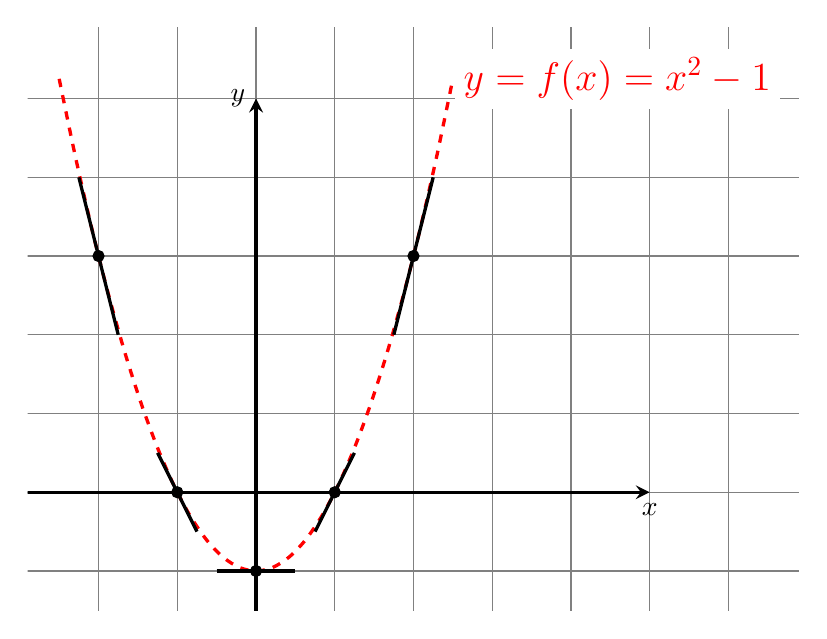
\begin{tikzpicture}[>=stealth]
\path[clip] (-2.9,-1.5) rectangle (6.9,5.9);
\draw[gray] (-6.9,-6.9) grid (6.9, 6.9);
\draw[very thick,->] (-5,0)--(5,0) node[below]{$x$};
\draw[very thick,->] (0,-5)--(0,5) node[left]{$y$};
\draw[very thick, red, dashed, domain=-2.5:2.5,smooth,variable=\t]
  plot ({\t},{\t*\t-1}) node[fill=white,right]{{\Large $y=f(x)=x^2-1$}};
\draw[very thick, domain=-0.5:0.5,variable=\t]
  plot ({\t},{-1});
\draw[very thick, domain=0.75:1.25,variable=\t]
  plot ({\t},{2*(\t-1)});
\draw[very thick, domain=1.75:2.25,variable=\t]
  plot ({\t},{3+4*(\t-2)});
\draw[very thick, domain=0.75:1.25,variable=\t]
  plot ({-\t},{2*(\t-1)});
\draw[very thick, domain=1.75:2.25,variable=\t]
  plot ({-\t},{3+4*(\t-2)});
\foreach \t in {-2,-1,0,1,2} {
\filldraw (\t,\t*\t-1) circle (2pt);
}
\end{tikzpicture}
\vspace{10mm}

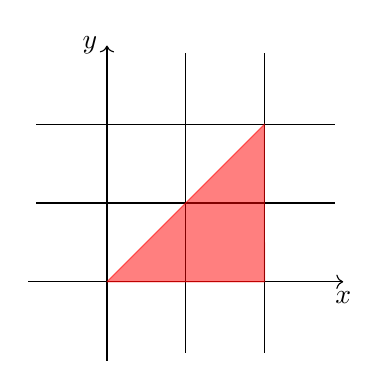
\begin{tikzpicture}
\draw (-0.9,-0.9) grid (2.9,2.9);
\draw[->] (-1,0)--(3,0) node[below]{$x$};
\draw[->] (0,-1)--(0,3) node[left]{$y$};
\filldraw[red,opacity=0.5] plot[domain=0:2](\x,\x)--(2,0)--(0,0);
\end{tikzpicture}
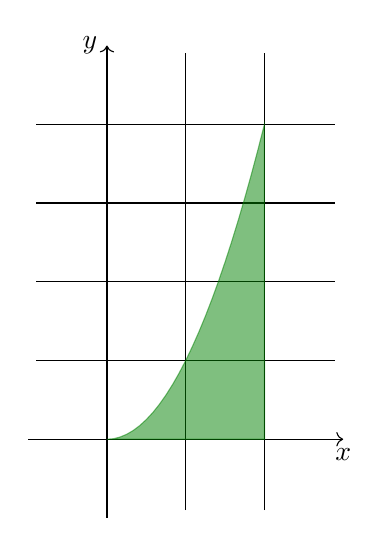
\begin{tikzpicture}
\draw (-0.9,-0.9) grid (2.9,4.9);
\draw[->] (-1,0)--(3,0) node[below]{$x$};
\draw[->] (0,-1)--(0,5) node[left]{$y$};
\filldraw[green!50!black,opacity=0.5] plot[domain=0:2](\x,\x*\x)--(2,0)--(0,0);
\end{tikzpicture}
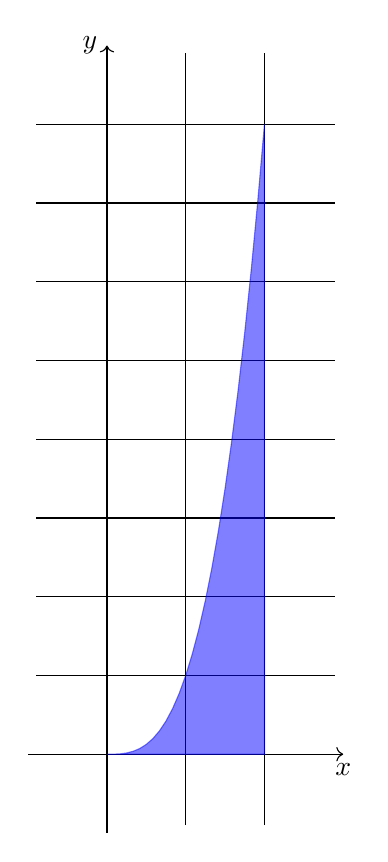
\begin{tikzpicture}
\draw (-0.9,-0.9) grid (2.9,8.9);
\draw[->] (-1,0)--(3,0) node[below]{$x$};
\draw[->] (0,-1)--(0,9) node[left]{$y$};
\filldraw[blue,opacity=0.5] plot[domain=0:2](\x,\x*\x*\x)--(2,0)--(0,0);
\end{tikzpicture}
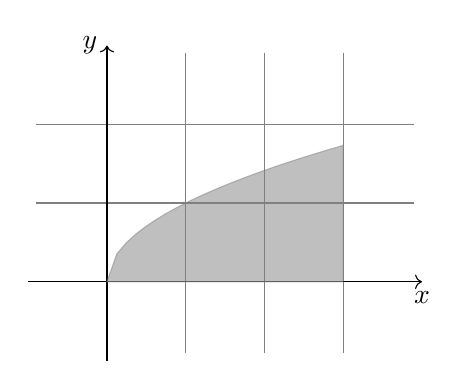
\begin{tikzpicture}
\draw[gray] (-0.9,-0.9) grid (3.9,2.9);
\draw[->] (-1,0)--(4,0) node[below]{$x$};
\draw[->] (0,-1)--(0,3) node[left]{$y$};
\filldraw[gray,opacity=0.5] plot[domain=0:3] (\x,{sqrt(\x)})--(3,0)--cycle;
\end{tikzpicture}

\section*{Esipuhe}

Materiaalissa tarkastellaan matematiikan tehtäviä aiheista derivaatta (=kasvunopeus) ja integraali (=pinta-alan kertymä). Materiaali koostuu pääosin esimerkeistä ja tehtävistä. Kaavojen todistuksia ei juurikaan ole.

Usein muissa materiaaleissa integrointia käsitellään vasta, kun derivointi on käsitelty\footnote{Lukion pitkässä matematiikassa on erilliset kurssit
\begin{itemize}
\item MAA6 Derivaatta (3 op)
\item MAA7 Integraalilaskenta (2 op)
\end{itemize}
lähde~\url{https://www.oph.fi/sites/default/files/documents/lukion\_opetussuunnitelman\_perusteet\_2019.pdf\#page=226}
}
Tästä poiketen, tässä materiaalissa pyritään tutustumaan viikoittain
\begin{itemize}
\setlength\itemsep{-0.5em}
\item alkeisfunktion derivaattaan
\item alkeisfunktion integraaliin
\item menetelmiin (monimutkaisemmat derivointisäännöt)
\item sovelluksiin
\item graafiseen puoleen
\end{itemize}
Materiaali on jaoteltu viikoittaisiin paketteihin - yksi funktiotyyppi viikkoa kohti. Etuna lienee, että jo kaksi ensimmäistä viikkoa antavat mielikuvan, mitä derivointi ja integrointi ovat. Lisäksi uusia kaavoja tulee tasaisemmin, kuin perinteisessä esitystavassa.

Materiaali oli käytössä keväällä 2024. Puutteita ja virheitä lienee sekä sisällössä että esitystavassa.\\

\noindent Oulussa 17.4.2024, Juha-Matti Huusko
\vspace{10mm}

Tämä moniste tarjotaan käyttöön lisenssillä \href{https://creativecommons.org/licenses/by-sa/4.0/legalcode.fi}{Nimeä-JaaSamoin 4.0 Kansainvälinen}

\tableofcontents

\newpage

\section{Lineaarinen funktio}

\subsection{Suoran yhtälö}

\textbf{Esimerkki.} Pisteiden $p=(1,2)$ ja $q=(4,3)$ kautta kulkevan suoran kulmakerroin on
$$
k=\frac{y_2-y_1}{x_2-x_1}=\frac{3-2}{4-1}=\frac{1}{3}.
$$
Pisteiden $p$ ja $q$ kautta kulkeva suora on
$$
y-y_1=k(x-x_1)
$$
eli
$$
y-2=\frac{1}{3}(x-1)
$$
eli normaalimuodossa $y=kx+b$ suoran yhtälö on $y=\frac13 x+\frac53$.

\def\px{1}
\def\py{2}
\def\qx{4}
\def\qy{3}
\begin{tikzpicture}
\path[clip] (-2.9,-1.9) rectangle (6,6);
\draw[gray] (-4.9,-4.9) grid (4.9, 4.9);
\draw[->] (-5,0)--(5,0) node[below]{$x$};
\draw[->] (0,-5)--(0,5) node[left]{$y$};
\filldraw (\px,\py) coordinate (p) circle (2pt) node[below right]{$p$};
\filldraw (\qx,\qy) coordinate (q) circle (2pt) node[below right]{$q$};
%\draw ($0.5*(p)+0.5*(q)$) circle (2pt);
\draw ($3*(p)-2*(q)$)--($-2*(p)+3*(q)$);
\draw[very thick] (p)--(p-|q)--(q);
\end{tikzpicture}

\newpage

\textbf{Tehtäviä.} Voit myös piirtää tehtävissä kuvat, jos haluat.

\begin{enumerate}
\item Tarkastellaan pisteiden $p=(1,3)$ ja $q=(4,2)$ kautta kulkevaa suoraa. 
%Piirrä pisteet ja niiden kautta kulkeva suora. 
Määritä suoran kulmakerroin ja suoran yhtälö normaalimuodossa.\ratkaisu{$k=-1/3$, $y=-\frac13 x+\frac{10}{3}$}
\item Tarkastellaan pisteiden $p=(1,2)$ ja $q=(4,2)$ kautta kulkevaa suoraa. 
%Piirrä pisteet ja niiden kautta kulkeva suora. 
Määritä suoran kulmakerroin ja suoran yhtälö normaalimuodossa.\ratkaisu{$k=0$, $y=2$}
\item Tarkastellaan pisteiden $p=(1,2)$ ja $q=(1.01,4)$ kautta kulkevaa suoraa. 
%Piirrä pisteet ja niiden kautta kulkeva suora. 
Määritä suoran kulmakerroin ja suoran yhtälö normaalimuodossa.\ratkaisu{$k=200$, $y=200x-198$}
\item Tarkastellaan suoraa $3y=2x+1$. Kirjoita yhtälö muodossa $y=kx+b$. Mikä on suoran kulmakerroin $k$? Etsi kaksi suoran pistettä. Piirrä suoran kuvaaja.
\ratkaisu{$y=\frac23 x+\frac13$, esim. $p=(1,1)$ ja $q=(4,3)$}
\item Määritä alla olevassa kuvassa pisteet $p$ ja $q$. Määritä suoran kulmakerroin ja suoran yhtälö normaalimuodossa.\ratkaisu{$y=-\frac12 x+\frac72$}
\end{enumerate}

\def\px{1}
\def\py{3}
\def\qx{3}
\def\qy{2}
\begin{tikzpicture}
\path[clip] (-2.9,-1.9) rectangle (6,6);
\draw[gray] (-4.9,-4.9) grid (4.9, 4.9);
\draw[->] (-5,0)--(5,0) node[below]{$x$};
\draw[->] (0,-5)--(0,5) node[left]{$y$};
\filldraw (\px,\py) coordinate (p) circle (2pt) node[below right]{$p$};
\filldraw (\qx,\qy) coordinate (q) circle (2pt) node[below right]{$q$};
%\draw ($0.5*(p)+0.5*(q)$) circle (2pt);
\draw ($3*(p)-2*(q)$)--($-2*(p)+3*(q)$);
\draw[very thick] (p)--(p-|q)--(q);
\end{tikzpicture}

\newpage

\subsection{Sijoitusmerkki}

Kurssilla opetellaan laskemaan pinta-aloja integroimalla tavalla
$$
\int_a^b f(x)dx\stackrel{(1)}{=}\sij_a^b F(x)\stackrel{(2)}{=}F(b)-F(a).
$$
Vaiheen (1) lasku riippuu siitä, mikä funktio $f$ on.

Harjoitellaan tällä viikolla vaihe (2) eli sijoitusmerkin käyttö. Sijoitettaessa lasketaan ``arvo ylärajalla miinus arvo alarajalla''.
$$
\sij_a^b F(x)=F(b)-F(a)
$$
Funktio $F(x)$ kertoo pinta-alan kertymän. Sijoitus
$$
\sij_a^b F(x)=F(b)-F(a)
$$
kertoo ``kuinka paljon lisää pinta-alaa välillä $[a,b]$ kertyi''.

\textbf{Esimerkki.} Lasketaan sijoitus
$$
\sij_2^5 x^2=5^2-2^2=25-4=21.
$$
\textbf{Esimerkki.} Lasketaan sijoitus
$$
\sij_2^5 \frac{1}{x}=\frac{1}{5}-\frac{1}{2}=\frac{2}{10}-\frac{5}{10}=-\frac{3}{10}.
$$
\textbf{Esimerkki.} Lasketaan sijoitus
$$
\sij_1^2 3x^2-x=(3\cdot 2^2-2)-(3\cdot 1^2-1)=(12-2)-(3-1)=8.
$$

\begin{enumerate}
\setcounter{enumi}{5}
\item Laske sijoitukset.
\begin{enumerate}
\item $\sij_3^4 x^2$\ratkaisu{$7$}
\item $\sij_3^4 \frac{1}{x}$\ratkaisu{$-\frac{1}{12}$}
\item $\sij_2^3 2x^2-x$\ratkaisu{$9$}
\item $\sij_2^6 \ln(x)$\ratkaisu{$\ln(3)$}
\item $\sij_0^\pi\cos(x)$\ratkaisu{$-2$}
\end{enumerate}\newpage
\item Laske alla olevien kuvien varjostetut pinta-alat. Riittää laskea sijoitukset. 
\end{enumerate}

\def\a{1}
\def\b{3}
\begin{tikzpicture}
\path[clip] (-0.9,-0.9) rectangle (6,6);
\draw[gray] (-4.9,-4.9) grid (4.9, 4.9);
\draw[->] (-5,0)--(5,0) node[below]{$x$};
\draw[->] (0,-5)--(0,5) node[left]{$y$};
\draw[very thick, red, domain=-5:5,smooth,variable=\t]
  plot ({\t},{2});
\draw[->] (-3.6,0)--(3.6,0);
\fill[opacity=0.5, gray, domain=\a:\b,smooth,variable=\t]
  plot ({\t},{2})--(\b,0)--(\a,0)--cycle;
%\filldraw (0,0) circle (2pt);
%\draw (0,0) node[below]{\Amu};
\filldraw (\a,0) circle (2pt);
\filldraw (\b,0) circle (2pt);
\draw (\a,0) node[below left]{\a};
\draw (\b,0) node[below right]{\b};
\end{tikzpicture}
$
\int_1^3 2dx=\sij_1^3 2x=
$

\def\a{1}
\def\b{3}
\begin{tikzpicture}
\path[clip] (-0.9,-0.9) rectangle (6,6);
\draw[gray] (-4.9,-4.9) grid (4.9, 4.9);
\draw[->] (-5,0)--(5,0) node[below]{$x$};
\draw[->] (0,-5)--(0,5) node[left]{$y$};
\draw[very thick, red, domain=-5:5,smooth,variable=\t]
  plot ({\t},{0.5*\t});
\draw[->] (-3.6,0)--(3.6,0);
\fill[opacity=0.5, gray, domain=\a:\b,smooth,variable=\t]
  plot ({\t},{0.5*\t})--(\b,0)--(\a,0)--cycle;
%\filldraw (0,0) circle (2pt);
%\draw (0,0) node[below]{\Amu};
\filldraw (\a,0) circle (2pt);
\filldraw (\b,0) circle (2pt);
\draw (\a,0) node[below left]{\a};
\draw (\b,0) node[below right]{\b};
\end{tikzpicture}
$
\int_1^3 0.5xdx=\sij_1^3 0.25x^2=
$

\def\a{1}
\def\b{3}
\begin{tikzpicture}
\path[clip] (-0.9,-0.9) rectangle (6,6);
\draw[gray] (-4.9,-4.9) grid (4.9, 4.9);
\draw[->] (-5,0)--(5,0) node[below]{$x$};
\draw[->] (0,-5)--(0,5) node[left]{$y$};
\draw[very thick, red, domain=-5:5,smooth,variable=\t]
  plot ({\t},{2+0.5*\t});
\draw[->] (-3.6,0)--(3.6,0);
\fill[opacity=0.5, gray, domain=\a:\b,smooth,variable=\t]
  plot ({\t},{2+0.5*\t})--(\b,0)--(\a,0)--cycle;
%\filldraw (0,0) circle (2pt);
%\draw (0,0) node[below]{\Amu};
\filldraw (\a,0) circle (2pt);
\filldraw (\b,0) circle (2pt);
\draw (\a,0) node[below left]{\a};
\draw (\b,0) node[below right]{\b};
\end{tikzpicture}$\int_1^3 2+0.5x dx=\sij_1^3 2x+0.25x^2=$

\newpage

\section{Polynomi}

\subsection{Monomin ja potenssin derivointi}

Monomia derivoidaan kaavalla $D x^n=nx^{n-1}$.

\textbf{Esimerkki.} Monomin $2x^7$ derivaatta on $2\cdot 7x^6=14x^6$. Toisin sanoin, jos $f(x)=2x^7$, niin $f'(x)=14x^6$.

\begin{enumerate}
\item Derivoi monomit.
\begin{enumerate}
\item $3x^5$\ratkaisu{$15x^4$}
\item $-3x^{11}$\ratkaisu{$-33x^{10}$}
\item $4x^1$\ratkaisu{$4$}
\item $2$ eli $2x^0$\ratkaisu{$0$}
\end{enumerate}
\end{enumerate}

%Vakion derivaatta on nolla eli $Da=0$ ja yksittäinen $x$ häviää derivoitaessa pois eli $Dax=a$, jos $a$ on vakio.

Derivointikaava $D x^n=nx^{n-1}$ toimii myös, kun $n$ on negatiivinen, murtoluku tai mikä tahansa luku. (Tällöin lauseke $x^n$ on muuttujan $x$ potenssi.)

\textbf{Esimerkki.} Lauseke $\dfrac{1}{x^3}$ voidaan kirjoittaa muodossa $x^{-3}$. Lausekkeen derivaatta on $-3x^{-3-1}=-3x^{-4}=\dfrac{-3}{x^4}$.

\textbf{Esimerkki.} Viidennen juuren $\sqrt[5]{x}$ voi kirjoittaa muodossa $x^{1/5}$. Tämän derivaatta on $\frac15x^{1/5-1}=\frac15x^{-4/5}$.

\textbf{Esimerkki.} $Dx^{3.1}=3.1x^{2.1}$

\begin{enumerate}
\setcounter{enumi}{1}
\item Derivoi muuttujan $x$ potenssit
\begin{enumerate}
\item $\dfrac{3}{x^2}$\ratkaisu{$-6x^{-3}$}
\item $\sqrt{x}$\ratkaisu{$\frac{1}{2\sqrt{x}}$}
\item $x\sqrt{x}$\ratkaisu{$\frac32\sqrt{x}$}
\item $2x^{-2.3}$\ratkaisu{$-4.6x^{-3.3}$}
\end{enumerate}
\end{enumerate}

\subsection{Polynomin derivointi}

Summan termejä derivoidaan erikseen ja edessä olevat vakiot säilyvät. %(Tästä syystä sanotaan, että derivaatta on \emph{lineaarinen} operaatio.)

Vakion derivaatta on nolla eli $Da=0$ ja yksittäinen $x$ häviää derivoitaessa pois eli $Dax=a$, jos $a$ on vakio

\textbf{Esimerkki.} Derivoidaan lauseketta $3x^2-2x^7+5x+3$. Saadaan
\begin{equation*}
\begin{split}
&D 3x^2-2x^7+5x+3\\
&=3\cdot 2x^1-2\cdot 7x^6+5+0.
\end{split}
\end{equation*}

\begin{enumerate}
\setcounter{enumi}{2}
\item Derivoi polynomit
\begin{enumerate}
\item $x^2-2x+1$\ratkaisu{$2x-2$}
\item $4x^3+7x-100$\ratkaisu{$12x^2+7$}
\item $5x^2-x+2$\ratkaisu{$10x-1$}
\item $x^4+x^3+x^2+x+1$\ratkaisu{$4x^3+3x^2+2x+1+0$}
\end{enumerate}
\end{enumerate}

\newpage

\subsection{Polynomin derivointi ja kuvaaja}

\begin{minipage}{0.45\linewidth}
\def\px{1}
\def\py{2}
\def\qx{4}
\def\qy{3}
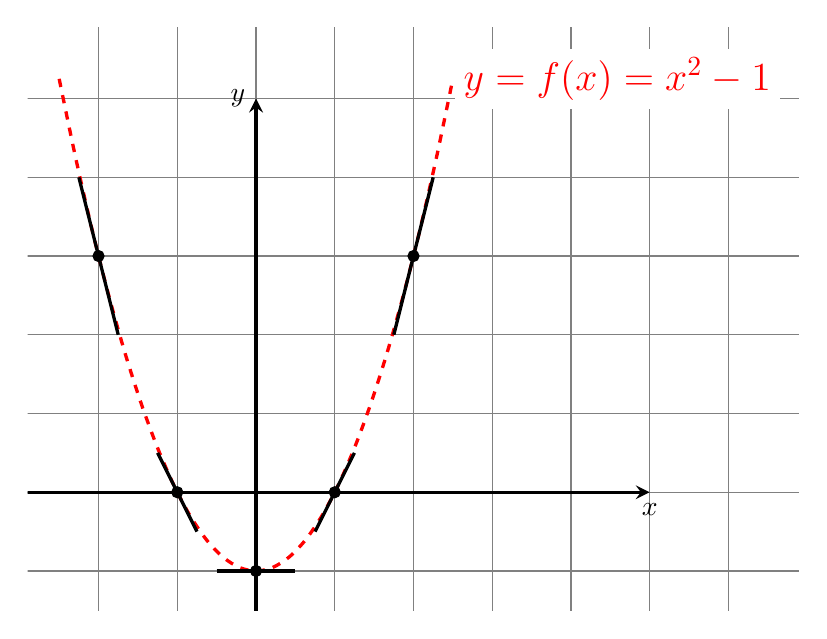
\begin{tikzpicture}[>=stealth]
\path[clip] (-2.9,-1.5) rectangle (6.9,5.9);
\draw[gray] (-6.9,-6.9) grid (6.9, 6.9);
\draw[very thick,->] (-5,0)--(5,0) node[below]{$x$};
\draw[very thick,->] (0,-5)--(0,5) node[left]{$y$};
\draw[very thick, red, dashed, domain=-2.5:2.5,smooth,variable=\t]
  plot ({\t},{\t*\t-1}) node[fill=white,right]{{\Large $y=f(x)=x^2-1$}};
\draw[very thick, domain=-0.5:0.5,variable=\t]
  plot ({\t},{-1});
\draw[very thick, domain=0.75:1.25,variable=\t]
  plot ({\t},{2*(\t-1)});
\draw[very thick, domain=1.75:2.25,variable=\t]
  plot ({\t},{3+4*(\t-2)});
\draw[very thick, domain=0.75:1.25,variable=\t]
  plot ({-\t},{2*(\t-1)});
\draw[very thick, domain=1.75:2.25,variable=\t]
  plot ({-\t},{3+4*(\t-2)});
\foreach \t in {-2,-1,0,1,2} {
\filldraw (\t,\t*\t-1) circle (2pt);
}
\end{tikzpicture}
\end{minipage}
\hfill
\begin{minipage}{0.45\linewidth}
\begin{enumerate}
\setcounter{enumi}{3}
\item Olkoon $f(x)=x^2-1$. Laske
\begin{enumerate}
\item $f'(x)$\ratkaisu{$2x$}
\item $f'(-2)$\ratkaisu{$-4$}
\item $f'(-1)$\ratkaisu{$-2$}
\item $f'(0)$\ratkaisu{$0$}
\item $f'(1)$\ratkaisu{$2$}
\item $f'(2)$\ratkaisu{$4$}
\end{enumerate}
\item Selvitä funktion $f(x)=x^2-1$ kuvaajalle pisteeseen $(1,0)$ piirretyn tangenttisuoran yhtälö.

\ratkaisu{$y-0=2(x-1)$}

\item Selvitä funktion $f(x)=x^2-1$ kuvaajalle pisteeseen $(0,-1)$ piirretyn tangenttisuoran yhtälö.

\ratkaisu{$y=-1$}

\item Selvitä funktion $f(x)=x^2-1$ kuvaajalle pisteeseen $(-2,3)$ piirretyn tangenttisuoran yhtälö.

\ratkaisu{$y-3=-4(x-(-2))$}
\end{enumerate}
\newpage
\end{minipage}
\vspace{2cm}

{\color{green!50!black}Ratkaisu.\\[2mm]

5. Tangenttisuoran yhtälön kaava on $y-y_1=k(x-x_1)$. Täytyy selvittää, mitä ovat $x_1$, $y_1$ ja $k$, ja sijoittaa arvot yhtälöön.\\

Nyt $(x_1,y_1)=(1,0)$, joten $x_1=1$ ja $y_1=0$.\\

Derivaatan avulla saadaan tangenttisuoran kulmakerroin $k$. Se on $k=f'(x_1)=f'(1)=2$. (Laskettiin tehtävässä 4.)\\

Sijoittamalla arvot saadaan $y-y_1=k(x-x_1)$ muotoon $y-0=2(x-1)$.

Jos halutaan, voidaan siistiä tämä muotoon $y=2x-2$.
}

\newpage

\begin{minipage}{0.45\linewidth}
\def\px{1}
\def\py{2}
\def\qx{4}
\def\qy{3}
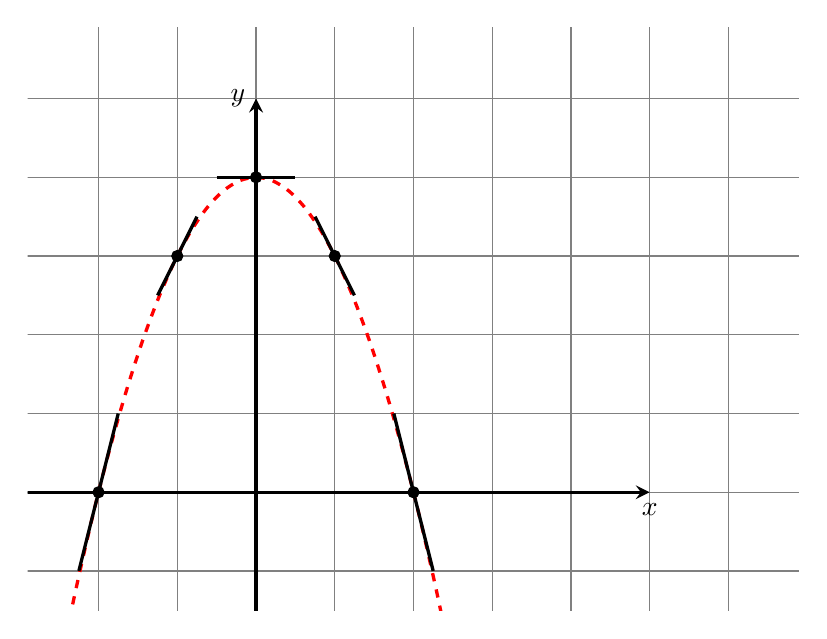
\begin{tikzpicture}[>=stealth]
\path[clip] (-2.9,-1.5) rectangle (6.9,5.9);
\draw[gray] (-6.9,-6.9) grid (6.9, 6.9);
\draw[very thick,->] (-5,0)--(5,0) node[below]{$x$};
\draw[very thick,->] (0,-5)--(0,5) node[left]{$y$};
\draw[very thick, red, dashed, domain=-2.5:2.5,smooth,variable=\t]
  plot ({\t},{-\t*\t+4}) node[fill=white,right]{{\Large $y=f(x)=x^2-1$}};
\draw[very thick, domain=-0.5:0.5,variable=\t]
  plot ({\t},{4});
\draw[very thick, domain=0.75:1.25,variable=\t]
  plot ({\t},{3-2*(\t-1)});
\draw[very thick, domain=1.75:2.25,variable=\t]
  plot ({\t},{-4*(\t-2)});
\draw[very thick, domain=0.75:1.25,variable=\t]
  plot ({-\t},{3-2*(\t-1)});
\draw[very thick, domain=1.75:2.25,variable=\t]
  plot ({-\t},{-4*(\t-2)});
\foreach \t in {-2,-1,0,1,2} {
\filldraw (\t,4-\t*\t) circle (2pt);
}
\end{tikzpicture}
\end{minipage}
\hfill
\begin{minipage}{0.45\linewidth}
\begin{enumerate}
\setcounter{enumi}{3}
\item Olkoon $f(x)=-x^2+4$. Laske
\begin{enumerate}
\item $f'(x)$\ratkaisu{$-2x$}
\item $f'(-2)$\ratkaisu{$4$}
\item $f'(-1)$\ratkaisu{$2$}
\item $f'(0)$\ratkaisu{$0$}
\item $f'(1)$\ratkaisu{$-2$}
\item $f'(2)$\ratkaisu{$-4$}
\end{enumerate}
\item Selvitä funktion $f(x)=-x^2+4$ kuvaajalle pisteeseen $(1,3)$ piirretyn tangenttisuoran yhtälö.

\ratkaisu{$y-3=-2(x-1)$}

\item Selvitä funktion $f(x)=-x^2+4$ kuvaajalle pisteeseen $(0,4)$ piirretyn tangenttisuoran yhtälö.

\ratkaisu{$y=4$}

\item Selvitä funktion $f(x)=-x^2+4$ kuvaajalle pisteeseen $(-2,0)$ piirretyn tangenttisuoran yhtälö.

\ratkaisu{$y-0=4(x-(-2))$}
\end{enumerate}
\end{minipage}

\newpage

\begin{multicols}{2}
\def\px{1}
\def\py{2}
\def\qx{4}
\def\qy{3}
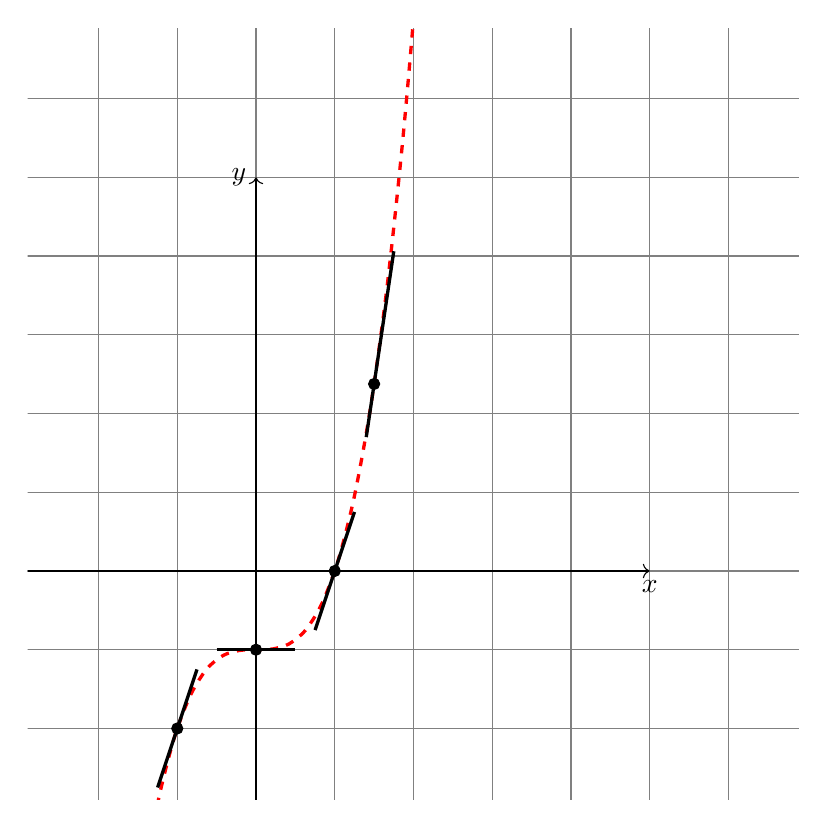
\begin{tikzpicture}
\path[clip] (-2.9,-2.9) rectangle (6.9,6.9);
\draw[gray] (-6.9,-6.9) grid (6.9, 6.9);
\draw[->] (-5,0)--(5,0) node[below]{$x$};
\draw[->] (0,-5)--(0,5) node[left]{$y$};
\draw[very thick, red, dashed, domain=-2.5:2.5,smooth,variable=\t]
  plot ({\t},{\t*\t*\t-1}) node[fill=white,right]{{\Large $y=f(x)=x^3-1$}};
\draw[very thick, domain=-0.5:0.5,variable=\t]
  plot ({\t},{-1});
\draw[very thick, domain=0.75:1.25,variable=\t]
  plot ({\t},{3*(\t-1)});
\draw[very thick, domain=1.4:1.75,variable=\t]
  plot ({\t},{2.375+6.75*(\t-1.5)});
\draw[very thick, domain=0.75:1.25,variable=\t]
  plot ({-\t},{-2-3*(\t-1)});
\foreach \t in {-1,0,1,1.5} {
\filldraw (\t,\t*\t*\t-1) circle (2pt);
}
\end{tikzpicture}
\vfill\null
\columnbreak
\begin{enumerate}
\setcounter{enumi}{3}
\item Olkoon $f(x)=x^3-1$. Laske
\begin{enumerate}
\item $f'(x)$\ratkaisu{$3x^2$}
\item $f'(-1)$\ratkaisu{$3$}
\item $f'(0)$\ratkaisu{$0$}
\item $f'(1)$\ratkaisu{$3$}
\item $f'(3/2)$\ratkaisu{$27/4$}
\end{enumerate}
\end{enumerate}
\end{multicols}

\subsection{Sovellus: ääriarvokohta (paikallinen minimi tai maksimi)}

Jos sileällä funktiolla $f(x)$ on paikallinen minimi tai maksimi jossakin pisteessä $x_0$, niin $f'(x_0)=0$. Siis derivaatan nollakohdat ovat mahdollisia minimi- tai maksimikohtia.

Yhteinen nimitys minimille tai maksimille on ääriarvo.

%Ääriarvokohdan paikallisuus tarkoittaa sitä

Tässä funktion sileys tarkoittaa sitä, että funktio on jatkuva (kuvaaja ei ole katkonainen) ja että funktio on derivoituva (kuvaajalla ei ole teräviä kärkiä).\\

\textbf{Esimerkki.} Etsitään funktion $f(x)=x^2-4x+7$ paikalliset ääriarvokohdat. Derivoimalla saadaan $f'(x)=2x-4$. Asetetaan derivaatta nollaksi, saadaan $2x-4=0$. Saadaan $x=2$. Koska funktion kuvaaja on ylöspäin aukeava paraabeli, kyseessä on paikallinen minimi. \textbf{Vastaus: paikallinen minimi kohdassa $x=2$.}

\begin{enumerate}
\setcounter{enumi}{7}
\item Olkoon $f(x)=3x^2+5x+13$. Etsi ääriarvokohdat.
\begin{enumerate}
\item Laske $f'(x)$.\ratkaisu{$f'(x)=6x+5$}
\item Kirjoita $f'(x)=0$. \ratkaisu{$6x+5=0$}
\item Ratkaise saadusta yhtälöstä $x$. \ratkaisu{$x=-\frac56$}
\item Voitko päätellä, onko kyseessä minimi vai maksimi?\ratkaisu{Minimi kohdassa $x=-\frac56$}
\end{enumerate}
\item Olkoon $f(x)=-3x^2+6x+2$. Etsi ääriarvokohdat.\ratkaisu{Maksimi kohdassa $x=1$}
%\begin{enumerate}
%\item Laske $f'(x)$.
%\item Kirjoita $f'(x)=0$.
%\item Ratkaise saadusta yhtälöstä $x$.
%\item Voitko päätellä, onko kyseessä minimi vai maksimi?
%\end{enumerate}
\item Olkoon $f(x)=x^2(1-x)$. Etsi ääriarvokohdat.
\begin{enumerate}
\item Avaa sulut.\ratkaisu{$f(x)=x^2-x^3$}
\item Laske $f'(x)$.\ratkaisu{$f'(x)=2x-3x^2$}
\item Kirjoita $f'(x)=0$.\ratkaisu{$2x-3x^2=0$}
\item Ratkaise saadusta yhtälöstä $x$.\ratkaisu{$x=0$ tai $x=\frac23$}
\item Voitko päätellä, onko kyseessä paikallinen minimi vai maksimi?\ratkaisu{Paikallinen minimi kohdassa $x=0$ ja paikallinen maksimi kohdassa $x=\frac23$.}
\end{enumerate}
\item Olkoon $f(x)=x^3(1-x)^2$. Etsi ääriarvokohdat.\ratkaisu{Paikallinen maksimi kohdassa $x=\frac{3}{5}$.}
\end{enumerate}

\newpage

\subsection{Potenssifunktion integrointi}

Integrointi on derivoinnille päinvastainen operaatio.

Derivoitaessa potenssifunktiota kerrotaan potenssilla ja uusi potenssi on yhtä pienempi, esimerkiksi $D x^5=5x^4$.

Toisaalta, integroitaessa potenssifunktiota uusi potenssi on yhtä suurempi ja sillä jaetaan, esimerkiksi $\int x^5dx=\frac{1}{6}x^6$.

Integrointia voidaan käyttää pinta-alan laskemiseen. Tällöin tarvitaan pinta-alan alkupiste $a$ ja loppupiste $b$. Vastaus saadaan sijoitusmerkin avulla
$$
\bigg /_a^b F(x)=F(b)-F(a).
$$
Esimerkiksi
$$
\int_2^3 x^7 dx=\bigg /_2^3 \frac{1}{8}x^8
=\frac{1}{8}3^8-\frac{1}{8}2^8.
$$

\begin{enumerate}
\setcounter{enumi}{7}
\item Laske integraalit.
\begin{enumerate}
\item $\int_0^2 xdx$\ratkaisu{$2$}
\item $\int_0^2 x^2dx$\ratkaisu{$\frac83$}
\item $\int_0^2 x^3dx$\ratkaisu{$4$}
\item $\int_0^3 \sqrt{x}dx$\ratkaisu{$2\sqrt{3}\approx 3.464.$}
\end{enumerate}
Integraalit kertovat eräiden tasoalueiden pinta-alat. Tasoalueet on piirretty alla oleviin kuviin.
\end{enumerate}

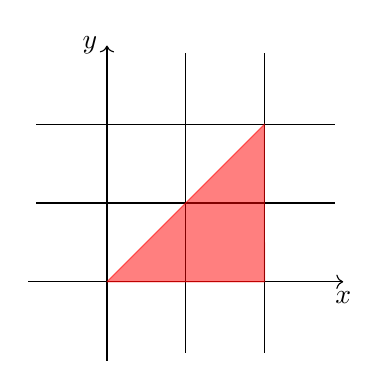
\begin{tikzpicture}
\draw (-0.9,-0.9) grid (2.9,2.9);
\draw[->] (-1,0)--(3,0) node[below]{$x$};
\draw[->] (0,-1)--(0,3) node[left]{$y$};
\filldraw[red,opacity=0.5] plot[domain=0:2](\x,\x)--(2,0)--(0,0);
\end{tikzpicture}
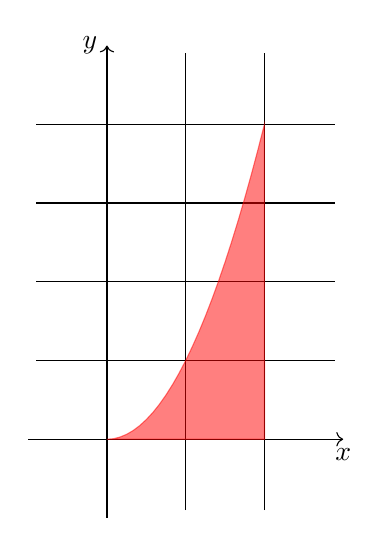
\begin{tikzpicture}
\draw (-0.9,-0.9) grid (2.9,4.9);
\draw[->] (-1,0)--(3,0) node[below]{$x$};
\draw[->] (0,-1)--(0,5) node[left]{$y$};
\filldraw[red,opacity=0.5] plot[domain=0:2](\x,\x*\x)--(2,0)--(0,0);
\end{tikzpicture}
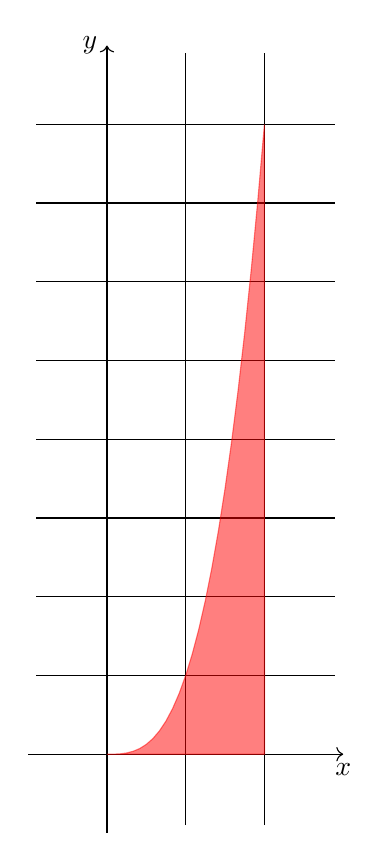
\begin{tikzpicture}
\draw (-0.9,-0.9) grid (2.9,8.9);
\draw[->] (-1,0)--(3,0) node[below]{$x$};
\draw[->] (0,-1)--(0,9) node[left]{$y$};
\filldraw[red,opacity=0.5] plot[domain=0:2](\x,\x*\x*\x)--(2,0)--(0,0);
\end{tikzpicture}
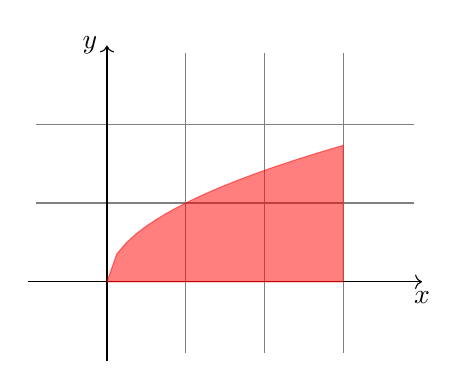
\begin{tikzpicture}
\draw[gray] (-0.9,-0.9) grid (3.9,2.9);
\draw[->] (-1,0)--(4,0) node[below]{$x$};
\draw[->] (0,-1)--(0,3) node[left]{$y$};
\filldraw[red,opacity=0.5] plot[domain=0:3] (\x,{sqrt(\x)})--(3,0)--cycle;
\end{tikzpicture}

\newpage

\section{Eksponenttifunktio}

\subsection{Eksponenttifunktion derivointi}

Eksponenttifunktiolle voidaan ottaa eri kantalukuja, esimerkiksi $2^x$, $3^x$, $1.1^x$. 

Yleisesti eksponenttifunktio on muotoa $a^x$, missä $a>0$. Pätee derivointikaava
$$
Da^x=a^x\ln(a).
$$

\textbf{Esimerkki.} Pätee $D8^x=8^x\ln(8)$.\\

Derivoidaan eksponenttifunktioita eri kantaluvuilla. Muista, että $a^0=1$ kaikilla $a>0$.
\begin{enumerate}
\item (\textbf{Laskettiin tunnilla! Ei tarvitse palauttaa.})Olkoon $f(x)=2^x$.
\begin{enumerate}
\item Laske $f'(x)$.\ratkaisu{$2^x\ln(2)$}
\item Laske $f'(0)$.\ratkaisu{$0.69$}
\end{enumerate}
\item Olkoon $g(x)=3^x$.
\begin{enumerate}
\item Laske $g'(x)$.\ratkaisu{$3^x\ln(3)$}
\item Laske $g'(0)$.\ratkaisu{$1.0986$}
\end{enumerate}
\item Olkoon $h(x)=1.1^x$.
\begin{enumerate}
\item Laske $h'(x)$.\ratkaisu{$1.1\ln(1.1)$}
\item Laske $h'(0)$.\ratkaisu{$0.095$}
\end{enumerate}
\item (\textbf{Laskettiin tunnilla! Ei tarvitse palauttaa.}) Olkoon $k(x)=0.5^x$.
\begin{enumerate}
\item Laske $k'(x)$.\ratkaisu{$0.5^x\ln(0.5)$}
\item Laske $k'(0)$.\ratkaisu{$-0.69$}
\end{enumerate}
\item Mikä tehtävien 1-4 funktioista kasvaa nopeimmin? Mikä funktioista kasvaa hitaimmin? Onko jokin funktioista jopa vähenevä?
\item Olkoon $m(x)=e^x$.
\begin{enumerate}
\item Laske $m'(x)$.\ratkaisu{$e^x\ln(e)$}
\item Laske $m'(0)$.\ratkaisu{$1$}
\end{enumerate}
\end{enumerate}

Jos eksponenttifunktion $a^x$ kantaluku on $a=e=2.71\ldots$, niin derivointikaavassa $\ln(a)=\ln(e)=1$ ja derivointikaava yksinkertaistuu muotoon
$$
De^x=e^x.
$$

\newpage
\subsection{Yhdistetyn funktion derivointi}

\textbf{Huom.} $a^{b^c}=a^{(b^c)}$ ja $(a^b)^c=a^{bc}$.\\

Usein monimutkaisen funktion voi ajatella koostuvan useista sisäkkäisistä funktioista.\\

\textbf{Esimerkki.} Funktio $e^{x^3}$ on $f(g(x)$, missä $f(x)=e^x$, $g(x)=x^3$.\\

Pätee yhdistetyn funktion derivoimiskaava
$$
Df(g(x))=f'(g(x))g'(x).
$$

\textbf{Esimerkki.} $D e^{x^3}=e^{x^3}\cdot Dx^3=e^{x^3}\cdot 3x^2$.

Lasketaan yhdistettyjen funktioiden derivaattoja. Saadaan samalla kertausta viime viikon asioista.

\begin{enumerate}
\setcounter{enumi}{6}
\item Laske
\begin{enumerate}
\item $De^{x^5}$\ratkaisu{$5x^4e^{x^5}$}
\item $D2^{x^5}$\ratkaisu{$5x^42^{x^5}\ln(2)$}
\item $De^{x^3+x^7}$
\ratkaisu{$De^{x^3+x^7}\cdot (3x^2+7x^6)$}
\item $De^{5x^3+x}$\ratkaisu{$e^{5x^3+x}\cdot (15x^2+1)$}
\item $De^{5x+1}$\ratkaisu{$5e^{5x+1}$}
\item $D2^{3x}$
\ratkaisu{$2^{3x}\cdot 3\cdot \ln(2)$}
\end{enumerate}
\item Laske
\begin{enumerate}
\item $De^{\sqrt{x}}$
\ratkaisu{$e^{\sqrt{x}}\cdot\frac{1}{2\sqrt{x}}$}
\item $De^{(1/x^2)}$\ratkaisu{$e^{(1/x^2)}\cdot\frac{-2}{x^3}$}
\item $D2^{(1/\sqrt{x})}$
\ratkaisu{$2^{(1/\sqrt{x})}\cdot\frac{-1}{2x\sqrt{x}}$}
\end{enumerate}
\end{enumerate}

\begin{enumerate}
\setcounter{enumi}{8}
\item Laske (Lähde: Kari Jyrkkä, Tekoäly on vaikea, vai onko?, video \url{https://www.youtube.com/watch?v=zgaw65VZZT8&t=295s}
\begin{enumerate}
\item $D2x^3$\ratkaisu{$6x^2
$}
\item $D(2x^3)^5$
\ratkaisu{$5\cdot (2x^3)^4\cdot 6x^2$}
\item $\frac{\partial}{\partial k}(2x^3+2k^2)^5$
\ratkaisu{$5(2x^3+2k^2)\cdot 4k^1$}
\end{enumerate}
\end{enumerate}

\newpage

\subsection{Eksponenttifunktion derivointi ja kuvaaja}

\begin{minipage}{0.45\linewidth}
\def\px{1}
\def\py{2}
\def\qx{4}
\def\qy{3}
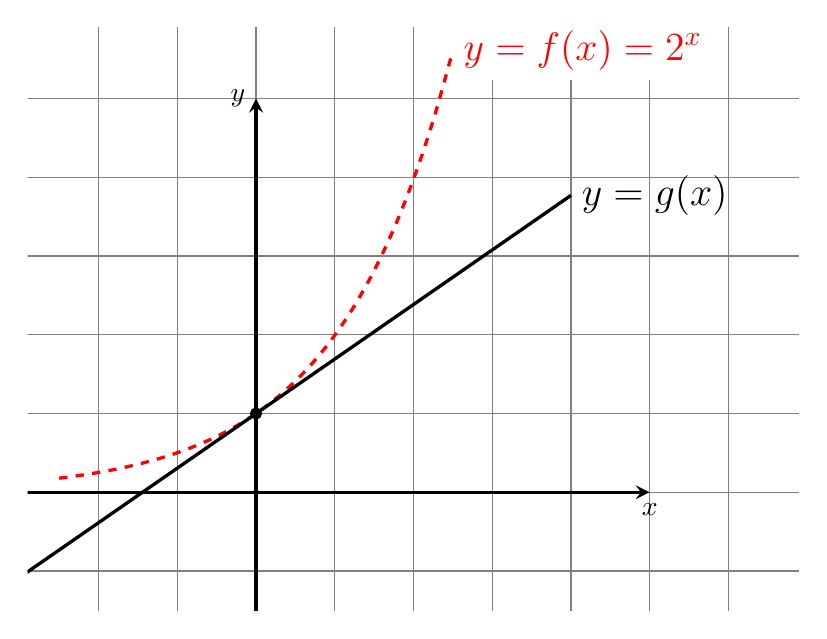
\begin{tikzpicture}[>=stealth]
\path[clip] (-2.9,-1.5) rectangle (6.9,5.9);
\draw[gray] (-6.9,-6.9) grid (6.9, 6.9);
\draw[very thick,->] (-5,0)--(5,0) node[below]{$x$};
\draw[very thick,->] (0,-5)--(0,5) node[left]{$y$};
%\draw[very thick, blue, domain=-2.5:2.5,smooth,variable=\t] plot ({\t},{1+0.693*\t+0.24*\t*\t});
\draw[very thick, red, dashed, domain=-2.5:2.5,smooth,variable=\t]
  plot ({\t},{exp(0.69*\t)}) node[fill=white,right]{{\Large $y=f(x)=2^x$}};
\draw[very thick] (-3,-1.08)--(4,3.77) node[right]{{\Large $y=g(x)$}};
\filldraw (0,1) circle (2pt);
\end{tikzpicture}\\[10mm]
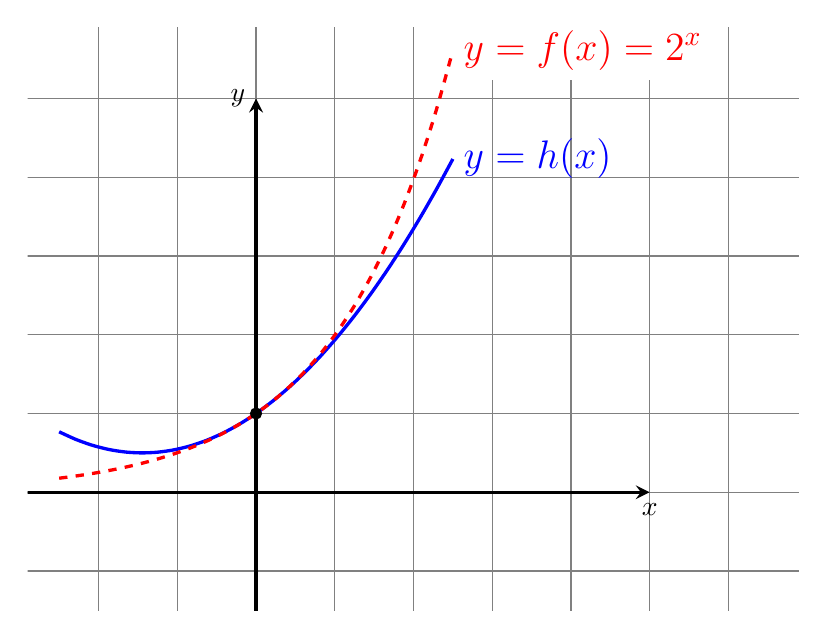
\begin{tikzpicture}[>=stealth]
\path[clip] (-2.9,-1.5) rectangle (6.9,5.9);
\draw[gray] (-6.9,-6.9) grid (6.9, 6.9);
\draw[very thick,->] (-5,0)--(5,0) node[below]{$x$};
\draw[very thick,->] (0,-5)--(0,5) node[left]{$y$};
\draw[very thick, blue, domain=-2.5:2.5,smooth,variable=\t]
  plot ({\t},{1+0.693*\t+0.24*\t*\t}) node[right]{{\Large $y=h(x)$}};
\draw[very thick, red, dashed, domain=-2.5:2.5,smooth,variable=\t]
  plot ({\t},{exp(0.69*\t)}) node[fill=white,right]{{\Large $y=f(x)=2^x$}};
%\draw[very thick] (-3,-1.08)--(5,4.46);
\filldraw (0,1) circle (2pt);
\end{tikzpicture}


\end{minipage}
\hfill
\begin{minipage}{0.45\linewidth}
\begin{enumerate}
\setcounter{enumi}{9}
\item Olkoon $f(x)=2^x$. Laske
\begin{enumerate}
\item $f'(x)$\ratkaisu{$2^x\ln(2)$}
\item $f'(0)$\ratkaisu{$\ln(2)\approx 0.7$}
\item $f'(1)$\ratkaisu{$1.4$}
\item $f'(2)$\ratkaisu{$2.8$}
\item $f'(-1)$\ratkaisu{$0.35$}
\item $f'(-2)$\ratkaisu{$0.175$}
\end{enumerate}
\item Selvitä funktion $f(x)=2^x$ kuvaajalle pisteeseen $(0,1)$ piirretyn tangenttisuoran 
\begin{enumerate}
\item kulmakerroin\ratkaisu{$\ln(2)\approx 0.7$}
\item yhtälö.\ratkaisu{$y=1+0.7x$}
\end{enumerate}

\item Olkoon\\ $f(x)=2^x$,\\  $g(x)=1+0.693x$, ja\\ $h(x)=1+0.693x+(0.693x)^2/2$.\\

Laske
\begin{enumerate}
\item $f(0.1)$\ratkaisu{$1.07177$}
\item $g(0.1)$\ratkaisu{$1.0693$}
\item $h(0.1)$\ratkaisu{$1.0717$}
\end{enumerate}
\end{enumerate}
\newpage
\end{minipage}

\newpage
\subsection{Sovellus: käännepiste}

Käännepiste tarkoittaa toisen derivaatan nollakohtaa. (Usein vaaditaan joitakin lisäehtoja, mutta sivuutetaan nämä.)

Siis $x_0$ on funktion $f(x)$ käännepiste, jos $f''(x_0)=0$.\\

\textbf{Esimerkki.} Funktiolle $f(x)=x^5+x^4$ ensimmäinen derivaatta on $f'(x)=5x^4+4x^3$ ja toinen derivaatta on
$$
f''(x)=20x^3+12x^2
=4x^2(5x+3)=0,
$$
jos $x=0$ tai $x=-3/5$. Käännepisteet ovat siis $x=0$ ja $x=-3/5$.

\begin{enumerate}
\setcounter{enumi}{12}
\item Etsi funktion $f(x)=x^3+x^2$ käännepisteet.
\begin{enumerate}
\item Laske $f'(x)$.
\item Laske $f''(x)$.\ratkaisu{$3x+2$}
\item Merkitse $f''(x)=0$ ja ratkaise $x$.\ratkaisu{$x=-2/3$}
\end{enumerate}
\item Etsi funktion $f(x)=e^{-x^2/2}$ käännepisteet.
\begin{enumerate}
\item Laske $f'(x)$.
\item Laske $f''(x)$.\ratkaisu{$e^{-x^2/2}(x^2-1)$}
\item Merkitse $f''(x)=0$ ja ratkaise $x$.\ratkaisu{$x=\pm1$}
\end{enumerate}
\end{enumerate}

\newpage

\subsection{Eksponenttifunktion integrointi}

Integrointi on derivoinnille päinvastainen operaatio.

Derivoitaessa eksponenttifunktiota kerrotaan kantaluvun logaritmilla $D a^x=a^x\ln(a)$, esimerkiksi $D2^x=2^x\ln(2)$.

Toisaalta, integroitaessa eksponenttifunktiota jaetaan kantaluvun logaritmilla, esimerkiksi $\int 2^x~dx=2^x\frac{1}{\ln(2)}$.

Integrointia voidaan käyttää pinta-alan laskemiseen. Tällöin tarvitaan pinta-alan alkupiste $a$ ja loppupiste $b$. Vastaus saadaan sijoitusmerkin avulla
$$
\bigg /_a^b F(x)=F(b)-F(a).
$$
Esimerkiksi
$$
\int_0^3 2^x dx=\bigg /_0^3 2^x/\ln(2)
=(1/\ln(2))\bigg /_0^3 2^x
=(1/\ln(2))(2^3-2^0)
=7/\ln(2).
$$

Yhdistetyn funktion integrointi ei aina onnistu. Esimerkiksi integraali
$$
\frac{1}{\sqrt{2\pi}}
\int_a^b e^{-x^2/2}~dx
$$
kertoo erään pinta-alan (normaalijakauman tiheysfunktion kertymä välillä $[a,b]$). Ei kuitenkaan ole suljettua kaavaa (kaava ilman sarjoja, integraalia, raja-arvoa jne.), kertoisi tämän luvun. 
\begin{enumerate}
\setcounter{enumi}{14}
\item Laske integraalit.
\begin{enumerate}
\item $\int_0^2 2^xdx$\ratkaisu{$4.3281$}
\item $\int_0^2 3^2dx$\ratkaisu{$7.2819$}
\item $\int_0^2 0.5^xdx$\ratkaisu{$1.082$}
\end{enumerate}
\item Laske sijoitukset. Integraalit kertovat eräiden tasoalueiden pinta-alat. Tasoalueet on piirretty alla oleviin kuviin.
\begin{enumerate}
\item $\int_0^2 e^x=\bigg/_0^2 e^x$\ratkaisu{$6.3891$}
\item $\int_0^1 e^{2x}dx=\bigg/_0^1 \frac{e^{2x}}{2}$\ratkaisu{$26.8$}
\item $\int_0^1 2x\cdot e^{x^2}=\bigg/_0^1 e^{x^2}$\ratkaisu{$1.7183$}
\end{enumerate}
\end{enumerate}

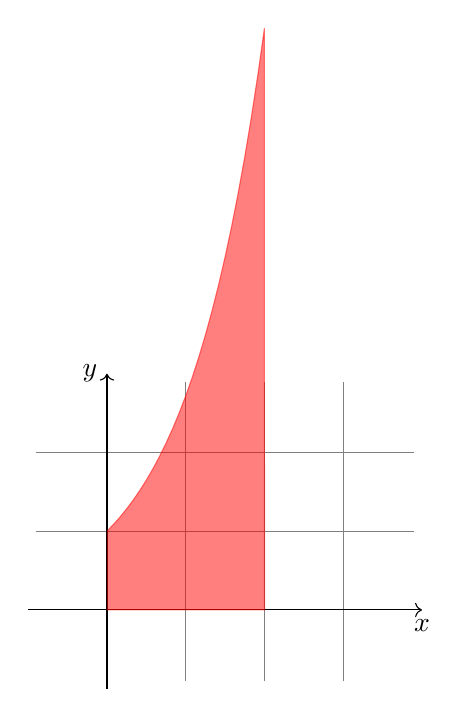
\begin{tikzpicture}
\draw[gray] (-0.9,-0.9) grid (3.9,2.9);
\draw[->] (-1,0)--(4,0) node[below]{$x$};
\draw[->] (0,-1)--(0,3) node[left]{$y$};
\filldraw[red,opacity=0.5] plot[domain=0:2] (\x,{exp(\x)})--(2,0)--(0,0);
\end{tikzpicture}
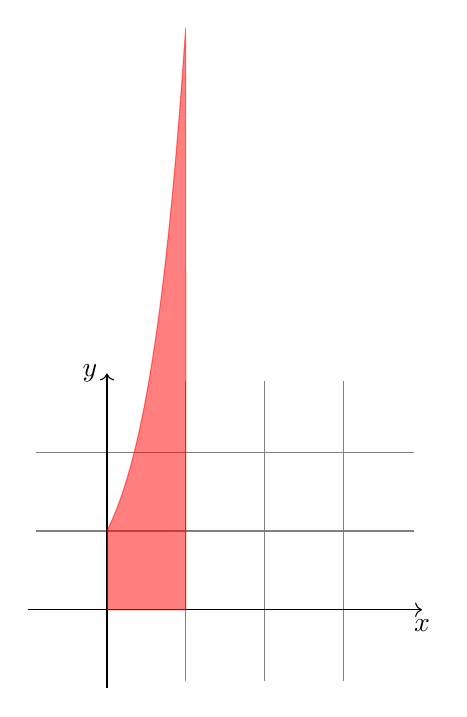
\begin{tikzpicture}
\draw[gray] (-0.9,-0.9) grid (3.9,2.9);
\draw[->] (-1,0)--(4,0) node[below]{$x$};
\draw[->] (0,-1)--(0,3) node[left]{$y$};
\filldraw[red,opacity=0.5] plot[domain=0:1] (\x,{exp(2*\x)})--(1,0)--(0,0);
\end{tikzpicture}
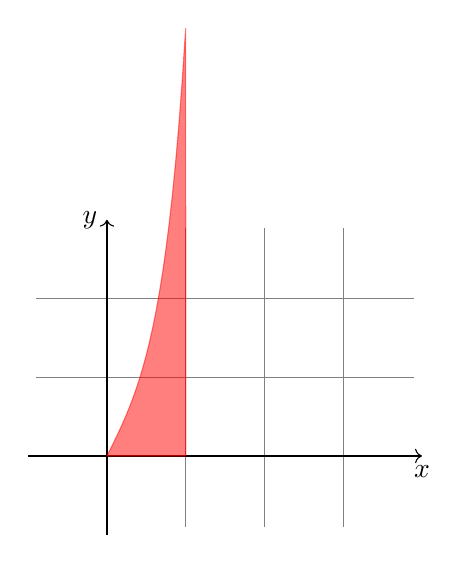
\begin{tikzpicture}
\draw[gray] (-0.9,-0.9) grid (3.9,2.9);
\draw[->] (-1,0)--(4,0) node[below]{$x$};
\draw[->] (0,-1)--(0,3) node[left]{$y$};
\filldraw[red,opacity=0.5] plot[domain=0:1] (\x,{2*\x*exp(\x*\x)})--(1,0)--(0,0);
\end{tikzpicture}

\newpage

\section{Logaritmifunktio}

Viime viikolla käsiteltiin eksponenttifunktion derivointia ja integrointia kaavoilla
\begin{equation*}
\label{eq:axderi}
Da^x=a^x\ln(a)
\quad\textrm{ja}\quad
\int a^xdx=\frac{a^x}{\ln(a)}.
\end{equation*}
Jos kantalukuna on $a=e$, niin kaavat yksinkertaistuvat.

Jos $x>0$, niin
$$
D\ln(x)=\frac{1}{x}
\quad\textrm{ja}\quad
\int \frac{1}{x}dx=\ln(x)
\quad\textrm{ja}\quad
\int \ln(x)dx=x\ln(x)-x.
$$
Muiden kantalukujen logaritmit voi muuttaa luonnolliseksi logaritmiksi eli $\log_a(x)=\frac{1}{\ln(a)}\ln(x)$

\subsection{Logaritmifunktion derivointi}

Jos logaritmin sisällä on jokin funktio, niin derivointi onnistuu kaavalla
$$
D\ln(f(x))=\frac{f'(x)}{f(x)}.
$$

\textbf{Esimerkki.}
$$
D\ln(x^2+3)=\dfrac{2x+0}{x^2+3}
$$

Jos logaritmin sisällä on jokin potenssi, niin ehkä on helpointa sieventää ennen derivointia kaavalla $\ln(x^n)=n\ln(x)$.

\textbf{Esimerkki.}
$$
D\ln(x^7)=D 7\ln(x)=\frac{7}{x}
$$

\textbf{Esimerkki.}
$$
D\sqrt[3](x^7)=D \ln(x^\frac{7}{3})=\frac{7}{3}D\ln(x)=\frac{7}{3}\ln(x).
$$

Derivoidaan logaritmifunktioita.

\begin{enumerate}
\item Laske
\begin{enumerate}
\item $D\ln(x^5)$\ratkaisu{$\frac{5}{x}$}
\item $D\log_2(x^5)$\ratkaisu{$\frac{1}{\ln(2)}\frac{5}{x}$}
\item $D\ln(x^3+x^7)$\ratkaisu{$\frac{3x^2+7x^6}{x^3+x^7}$}
\item $D\ln(5x^3+x)$\ratkaisu{$\frac{15x^2+1}{5x^3+x}$}
\item $D\ln(5x+1)$\ratkaisu{$\frac{5}{5x+1}$}
\item $D\log_2(3x)$
\ratkaisu{$\frac{1}{\ln(2)}\frac{3}{x}$}
\end{enumerate}
\item Laske
\begin{enumerate}
\item $D\ln(\sqrt{x})$\ratkaisu{$\frac{1}{2}\frac{1}{x}$}
\item $D\ln(1/x^2)$\ratkaisu{$-2\frac{1}{x}$}
\item $D\log_2(1/\sqrt{x})$
\ratkaisu{$\frac{1}{\ln(2)}\frac{1}{2}\frac{1}{x}$}
\end{enumerate}
\end{enumerate}

\newpage

\subsection{Logaritmifunktion derivointi ja kuvaaja}

\begin{minipage}{0.45\linewidth}
\def\px{1}
\def\py{2}
\def\qx{4}
\def\qy{3}
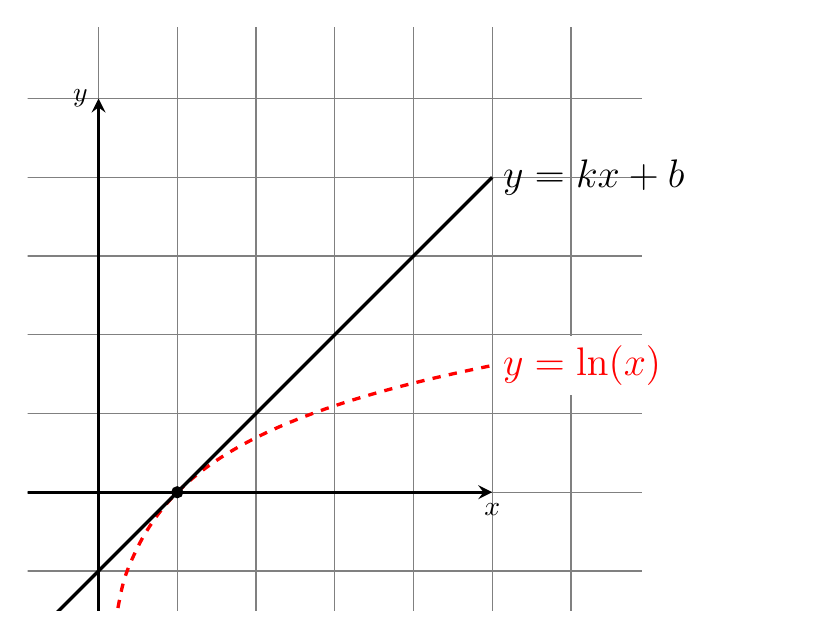
\begin{tikzpicture}[>=stealth]
\path[clip] (-0.9,-1.5) rectangle (8.9,5.9);
\draw[gray] (-6.9,-6.9) grid (6.9, 6.9);
\draw[very thick,->] (-5,0)--(5,0) node[below]{$x$};
\draw[very thick,->] (0,-5)--(0,5) node[left]{$y$};
%\draw[very thick, blue, domain=-2.5:2.5,smooth,variable=\t] plot ({\t},{1+0.693*\t+0.24*\t*\t});
\draw[very thick, red, dashed, domain=0.1:5,smooth,variable=\t]
  plot ({\t},{ln(\t)}) node[fill=white,right]{{\Large $y=\ln(x)$}};
\draw[very thick] (-1,-2)--(5,4) node[right]{{\Large $y=kx+b$}};
\filldraw (1,0) circle (2pt);
\end{tikzpicture}


\end{minipage}
\hfill
\begin{minipage}{0.45\linewidth}
\begin{enumerate}
\setcounter{enumi}{2}
\item Olkoon $f(x)=\ln(x)$. Laske
\begin{enumerate}
\item $f'(x)$\ratkaisu{$\frac{1}{x}$}
\item $f'(1)$\ratkaisu{$1$}
\item $f'(2)$\ratkaisu{$0.5$}
\item $f'(3)$\ratkaisu{$0.33$}
\item $f'(4)$\ratkaisu{$0.25$}
\item $f'(5)$\ratkaisu{$0.2$}
\end{enumerate}
\item Selvitä funktion $f(x)=\ln(x)$ kuvaajalle pisteeseen $(1,0)$ piirretyn tangenttisuoran 
\begin{enumerate}
\item kulmakerroin\ratkaisu{$1$}
\item yhtälö.\ratkaisu{$y=x-1$}
\end{enumerate}
\end{enumerate}
\end{minipage}

\newpage

\subsection{Funktion potenssin integrointi}

Aiemmin nähtiin
$$
Dx^n=nx^{n-1}
\quad\textrm{ja}\quad
\int x^ndx=\frac{1}{n+1}x^{n+1}, n\neq 1.
$$
Jos kyseessä on yhdistetty funktio, niin
$$
D f(x)^n=nf(x)^{n-1}f'(x)
\quad\textrm{ja}\quad
\int f(x)^nf'(x)dx=\frac{1}{n+1}f(x)^{n+1}, n\neq 1.
$$
Yllä olevissa integrointikaavoissa ei voida laittaa $n=-1$, koska silloin jaettaisiin nollalla. Potenssia $n=-1$ vastaa integrointikaava
$$
\int\frac{f'(x)}{f(x)}dx=\ln(f(x)).
$$

\textbf{Esimerkki.}
$$
\int 3x^2(x^3+1)^5dx=\frac{1}{6}(x^3+1)^6
$$
$$
\int \frac{3x^2}{(x^3+1)^5}dx=\frac{1}{-4}\frac{1}{(x^3+1)^4}
$$
$$
\int \frac{3x^2}{x^3+1}dx=\ln(x^3+1)
$$


\begin{enumerate}
\setcounter{enumi}{4}
\item Laske integraalit
\begin{enumerate}
\item $\int 2x(x^2+1)^3dx$\ratkaisu{$\frac{1}{4}(x^2+1)^4$}
\item $\int\dfrac{2x}{(x^2+1)^3}$\ratkaisu{$\frac{1}{-2}\frac{1}{(x^2+1)^2}$}
\item $\int\dfrac{2x}{x^2+1}dx$\ratkaisu{$\ln(x^2+1)$}
\end{enumerate}
\item Laske integraalit
\begin{enumerate}
\item $\int\dfrac{5x^4+1}{x^5+x}dx$
\item $\int (5x^4+1)(x^5+x)^7dx$
\item $\int (5x^4+1)\sqrt{x^5+x}dx$
\end{enumerate}
\end{enumerate}

\newpage
\section{Trigonometriset funktiot}
\subsection{Sinin ja kosinin derivaatta}

Sinin derivaatta on kosini eli $D\sin(x)=\cos(x)$.

Kosinin derivaatta on sini $D\cos(x)=-\sin(x)$. (Jos kosahtaa, se on miinus sinulta.)\\[2mm]

\textbf{Esimerkki.} $D\sin(3x+2)=\cos(3x+2)D(3x+2)=\cos(3x+2)\cdot (3+0)=3\cos(3x+2)$.

\begin{enumerate}
\item Laske derivaatta.
\begin{enumerate}
\item $f(x)=\sin(7x)$\ratkaisu{$f'(x)=7\cos(7x)$}
\item $g(x)=\cos(7x)$\ratkaisu{$g'(x)=-7\sin(7x)$}
\item $h(x)=\sin(2-3x)$\ratkaisu{$h'(x)=-3\cos(2-3x)$}
\end{enumerate}    
\end{enumerate}
\textbf{Esimerkki.} $D\sin(x^3)=\cos(x^3)\cdot 3x^2$.

\begin{enumerate}
\setcounter{enumi}{1}
\item Laske derivaatta.
\begin{enumerate}
\item $f(x)=\sin(x^7)$\ratkaisu{$f'(x)=7x^6\cos(x^7)$}
\item $g(x)=\cos(x^7)$\ratkaisu{$g'(x)=-7x^6\sin(x^7)$}
\item $h(x)=\sin(x^{-3})$\ratkaisu{$h'(x)=-3x^{-4}\cos(x^{-3})$}
\end{enumerate}    
\end{enumerate}
\textbf{Esimerkki.}
\begin{equation*}
\begin{split}
D2e^{5\sin(3x)}
&=2De^{5\sin(3x)}\\
&=2e^{5\sin(3x)}\cdot D(5\sin(3x))\\
&=10e^{5\sin(3x)}D\sin(3x)\\
&=10e^{5\sin(3x)}\cdot\cos(3x)\cdot 3\\
&=30e^{5\sin(3x)}\cos(3x)
\end{split}
\end{equation*}


\begin{enumerate}
\setcounter{enumi}{2}
\item Laske derivaatta.
\begin{enumerate}
\item $f(x)=2e^{\sin(7x)}$\ratkaisu{$f'(x)=14e^{\sin(7x)}\cos(7x)$}
\item $g(x)=3e^{2\cos(2x)}$\ratkaisu{$g'(x)=-12e^{2\cos(2x)}\sin(2x)$}
\item $h(x)=-2e^{-\cos(5x)}$\ratkaisu{$h'(x)=-10e^{-\cos(5x)}\sin(5x)$}
\end{enumerate}    
\end{enumerate}
\textbf{Huomautus.} Merkintä $\sin^3(x)$ tarkoittaa samaa kuin $(\sin(x))^3$. Merkinnän etu on siinä, että tarvitaan vähemmän sulkuja. Merkintää käytetään yleensä vain kokonaisluvuille.\\[2mm]
\textbf{Esimerkki.} $D\sin^5(x)=5\sin^4(x) D\sin(x)=5\sin^4(x)\cos(x)$

\begin{enumerate}
\setcounter{enumi}{3}
\item Derivoi
\begin{enumerate}
\item $D\sin^7(x)$\ratkaisu{$7\sin^6(x)\cos(x)$}
\item $D\cos^3(x)$\ratkaisu{$-3\cos^2(x)\sin(x)$}
\item $D\sin^5(2x)$\ratkaisu{$10\sin^4(2x)\cos(2x)$}
\item $D\frac{1}{\sin^2(3x)}$\ratkaisu{$-6(\sin(3x))^{-3}\cos(3x)$}
\item $D\sqrt{\cos(4x)}$\ratkaisu{$-2(\cos(4x))^{-1/2}\sin(4x)$}
\end{enumerate}
\end{enumerate}

\newpage

\subsection{Tulon ja osamäärän derivaatta}

Kahden funktion tulon derivaatan voi laskea kaavalla\footnote{\textbf{Perustelu.} Funktioilla on lineaariset approksimaatiot
\begin{equation*}
\begin{split}
f(x+h)&\approx f(x)+f'(x)h\\
g(x+h)&\approx g(x)+g'(x)h,\quad\textrm{kun}\quad h\to 0.\\
\end{split}
\end{equation*}
Tulon lineaarinen approksimaatio on
\begin{equation*}
\begin{split}
f(x+h)g(x+h)
&\approx (f(x)+f'(x)h)(g(x)+g'(x)h)\\
&=f(x)g(x)+[f'(x)g(x)+f(x)g'(x)]h
+f'(x)g'(x)h^2\\
&\approx f(x)g(x)+[f'(x)g(x)+f(x)g'(x)]h,\quad\textrm{kun}\quad h\to 0.
\end{split}
\end{equation*}}
$$
D(fg)=gDf+fDg.
$$
Kahden funktion osamäärän derivaatan voi laskea kaavalla\footnote{\textbf{Perustelu.} Kaavan voi johtaa laskemalla derivaatan $Df(x)g(x)^{-1}$ tulon derivaatan kaavalla.}
$$
D\frac{f}{g}=\frac{gDf-fDg}{g^2}.
$$
\textbf{Esimerkki.} $Dx^3\sin(5x)=3x^2\cdot \sin(5x)+x^3\cdot 5\cos(5x)$

\begin{enumerate}
\setcounter{enumi}{4}
\item Derivoi
\begin{enumerate}
\item $Dx^7\cos(2x)$
\item $Dx^3e^{x}$
\item $Dx^5\ln(x)$
\item $D\sin(x)\ln(x)$
\item $De^{2x}\cos(3x)$
\end{enumerate}
\end{enumerate}
\textbf{Esimerkki.}
$$
D\frac{x^3}{\sin(5x)}=\frac{3x^2\cdot \sin(5x)+x^3\cdot 5\cos(5x)}{\sin^2(5x)}
$$

\begin{enumerate}
\setcounter{enumi}{5}
\item Derivoi
\begin{enumerate}
\item $D\dfrac{x^7}{\cos(2x)}$
\item $D\dfrac{x^3}{e^{x}}$
\item $D\dfrac{x^5}{\ln(x)}$
\item $D\dfrac{\sin(x)}{\ln(x)}$
\item $D\dfrac{e^{2x}}{\cos(3x)}$
\end{enumerate}
\end{enumerate}

Tangenttifunktio ja kotangenttifunktio ovat
$$
\tan(x)=\frac{\sin(x)}{\cos(x)},\quad \cot(x)=\frac{\cos(x)}{\sin(x)}
$$

\begin{enumerate}
\setcounter{enumi}{6}
\item Laske $D\tan(x)=D\dfrac{\sin(x)}{\cos(x)}$.\ratkaisu{$\dfrac{\cos^2(x)+\sin^2(x)}{\cos^2(x)}=\frac{1}{\cos^2(x)}$}
\item Laske $D\cot(x)=D\dfrac{\cos(x)}{\sin(x)}$.\ratkaisu{$\dfrac{-\cos^2(x)-\sin^2(x)}{\cos^2(x)}=-\frac{1}{\sin^2(x)}$}
\item Laske $D\ln(\sin(2x))$.\ratkaisu{$\dfrac{2\cos(2x)}{\sin(2x)}$}
\item Laske $D\ln(2\cos(2x))$.\ratkaisu{$\dfrac{-\sin(2x)}{\cos(2x)}$}
\end{enumerate}

\newpage

\subsection{Sovellus: käämi ja kondensaattori}

Jos käämin läpi kulkevaa virtaa muutetaan, muutos tapahtuu viiveellä.
\begin{itemize}
\item Syy, lyhyesti: käämi vastustaa virran muutoksia.
\item Syy, pidemmästi: kun virta muuttuu, sen tuottaman magneettikentän vuo käämin läpi muuttuu, mikä aiheuttaa käämiin induktiojännitteen, joka vaikuttaa varausten liikkeeseen eli virtaan.
\end{itemize}
Käämille (eli kelalle)
$$
u(t)=-L\frac{d}{dt}i(t).
$$
Tässä
\begin{itemize}
\item $t$ on aika, yksikkö [s]
\item $i(t)$ on käämin läpi kulkeva virta hetkellä $t$, yksikkö [mA]
\item $L$ on käämin induktanssi, yksikkö [H] ``henry''
\item $u(t)$ on käämin tuottama induktiojännite, yksikkö [V]
\item miinusmerkki liittyy siihen, että käämi vastustaa virran muutosta
\item yksiköille V=H*A
\end{itemize}
\textbf{Esimerkki.}  Vaihtovirtapiirissä on virta $i(t)=5\sin(50\cdot 2\pi t)$~mA. (Virran taajuus on $50$~Hz ``hertzi''.) Virta kulkee käämin\footnote{esim. \url{https://www.spelektroniikka.fi/p23721-kuristin-suurille-virroille-n-200uh-fi.html}} (induktanssi $L=0.0002$~H) läpi. Laske käämin napojen välinen maksimijännite olettaen, että käämin resistanssi on nolla.\\

\noindent\textbf{Ratkaisu.} Virran derivaatta on
$$
\frac{d}{dt}i(t)
=\frac{d}{dt} 5\sin(100\pi t)
=500\pi\cos(100\pi t)~\textrm{mA/s}.
$$
Saadaan
$$
u(t)=-L\frac{d}{dt}i(t)
=-0.0002\cdot 500\pi\cos(100\pi t)~\textrm{H mA/s}
=-0.1\cos(100\pi t)~\textrm{mV}.
$$
Kosinin maksimiarvo on $1$. Siis $u(t)$:n maksimi on $0.1$~mV.\\[2mm]

Kondensaattorin latautuessa tai purkautuessa kulkee virta, jonka suuruus on
$$
i(t)
=C\frac{d}{dt}u(t).
$$
Tässä $C$ on kondensaattorin kapasitanssi, yksikkö F ``faradi''. Yksiköille A=F*V.

\textbf{Pari tehtävää.} 
\begin{enumerate}
\setcounter{enumi}{10}
\item Ison kondensaattorin\footnote{esim. \url{https://www.radioduo.fi/elektroniikka/elektrolyyttikondensaattori-tht-1000uf-50vdc-200-kpl/p/UKZ1H102MHM/}} (kapasitanssi $C=0.001~\textrm{F}$) napojen välinen jännite on
$$
u(t)=15e^{-t}~\textrm{mV}.
$$
Laske kondensaattorin läpi kulkeva virta hetkellä $t=1~\textrm{s}$.
\ratkaisu{$0.015e^{-1}\approx 0.0055$~mA}
\item Vaihtovirtapiirissä on virta $i(t)=5\sin(5000\cdot 2\pi t)$~mA. Virta kulkee käämin (induktanssi $L=0.0002$~H) läpi. Laske käämin napojen välinen maksimijännite olettaen, että käämin resistanssi on nolla.\ratkaisu{$10$~V}
\end{enumerate}

\newpage
\subsection{Funktion potenssin integrointi}

Aiemmin nähtiin
$$
\begin{array}{rl|rl}
\textbf{Derivointi} && \textbf{Integrointi}&\\[2mm]
Dx^n&=nx^{n-1}     \qquad\qquad&\qquad\qquad
\int x^ndx&=\frac{x^{n+1}}{n+1},\quad n\neq 1,\\[2mm]
D\ln(x)&=\frac{1}{x} &
\int\frac{1}{x}dx&=\ln(x)\\[2mm]
\end{array}
$$
Vastaavat yhdistetyn funktion kaavat
$$
\begin{array}{rl|rl}
\textbf{Derivointi} && \textbf{Integrointi}&\\[2mm]
Df(x)^n&=nf(x)^{n-1}f'(x)     \qquad\qquad&\qquad\qquad
\int f(x)^nf'(x)dx&=\frac{f(x)^{n+1}}{n+1},\quad n\neq 1,\\[2mm]
D\ln(f(x))&=\frac{f'(x)}{f(x)} &
\int\frac{f'(x)}{f(x)}dx&=\ln(f(x))\\[2mm]
\end{array}
$$

\textbf{Esimerkki.}
Integraali
$$
\int \cos(x)(\sin(x))^5dx=\frac{1}{6}(\sin(x))^6
$$
onnistui suoraan. Integraalissa
$$
\int \frac{\sin(x)}{(\cos(x))^5}dx=-\int \frac{-\sin(x)}{(\cos(x))^5}dx=-\frac{1}{-4}\frac{1}{(\cos(x))^4}
$$
piti saada puuttuva miinus integraalin sisälle. Integraalissa
$$
\int \frac{\cos(7x)}{\sin(7x)}dx
=
\frac{1}{7}\int \frac{7\cos(7x)}{\sin(7x)}dx=\ln(\sin(x))
$$
piti saada puuttuva $7$ integraalin sisälle.

\begin{enumerate}
\setcounter{enumi}{12}
\item Laske integraalit
\begin{enumerate}
\item $\int \sin(x)(\cos(x))^3dx$\ratkaisu{$-\frac{1}{4}(\cos(x))^4$}
\item $\int\dfrac{\cos(x)}{(\sin(x))^3}$\ratkaisu{$\frac{1}{-2}\frac{1}{(\sin(x))^2}$}
\item $\int\dfrac{\cos(x)}{\sin(x)}dx$\ratkaisu{$\ln(\sin(x))$}
\end{enumerate}
\item Laske integraalit
\begin{enumerate}
\item $\int (\cos(x))^3(\sin(x))^7dx$
\vihje{Sijoita $(\cos(x))^3=\cos(x)-\cos(x)(\sin(x))^2$.}

\item $\int \tan(x)dx$
\vihje{Sijoita $\tan(x)=\dfrac{\sin(x)}{\cos(x)}$.}
\item $\int \sin(x)\sqrt{\cos(x)}dx$
\vihje{Muista $\sqrt{a}=a^{1/2}$.}
\item $\int 2\sin(7x)\sin(3x)dx$
\vihje{Käytä kaavaa $2\sin(a)\sin(b)=\cos(a-b)-\cos(a+b)$}
\end{enumerate}
\end{enumerate}

\newpage
\subsection{Sinin ja kosinin integrointi}

\textbf{Esimerkki.} Käyrän $y=\sin(x)$, suoran $y=0$ (siis $x$-akseli) ja suorien $x=0$ ja $x=\pi/4$ rajaama pinta-ala on
$$
\int_0^{\pi/4}\sin(x)dx
=\bigg/_0^{\pi/4}-\cos(x)
=-\cos(\pi/4)-(-\cos(0))
=-\frac{1}{\sqrt{2}}+1\approx 0.292893.
$$

\begin{enumerate}
\setcounter{enumi}{14}
\item Laske määrätyt integraalit. Kuvat vastaavista pinta-aloista löytyvät alta. Punainen pinta-ala lasketaan positiivisena ja sininen pinta-ala negatiivisena.
\begin{enumerate}
\item $$
\int_0^\pi \sin(x)dx
$$
\item 
$$
\int_{-\frac{\pi}{2}}^{\frac{\pi}{2}} \cos(x)dx
$$
\item 
$$
\int_0^{2\pi} \sin(x)dx
$$
\end{enumerate}
\end{enumerate}

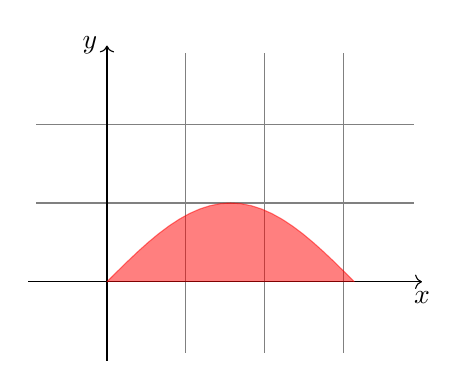
\begin{tikzpicture}
\draw[gray] (-0.9,-0.9) grid (3.9,2.9);
\draw[->] (-1,0)--(4,0) node[below]{$x$};
\draw[->] (0,-1)--(0,3) node[left]{$y$};
\filldraw[red,opacity=0.5] plot[domain=0:3.1415] (\x,{sin(180*\x/3.1415)});
\end{tikzpicture}
%$\int_0^\pi \sin(x)dx=\bigg /_0^\pi -\cos(x)=$
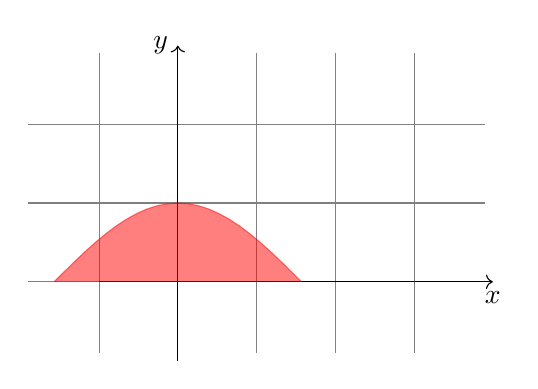
\begin{tikzpicture}
\draw[gray] (-1.9,-0.9) grid (3.9,2.9);
\draw[->] (-1,0)--(4,0) node[below]{$x$};
\draw[->] (0,-1)--(0,3) node[left]{$y$};
\filldraw[red,opacity=0.5] plot[domain=-1.57:1.57] (\x,{cos(90*\x/1.57)});
\end{tikzpicture}\\[2mm]
%$\int_{-\frac{\pi}{2}}^{\frac{\pi}{2}} \cos(x)dx=\bigg /_{-\pi/2}^{\pi/2} \sin(x)=$

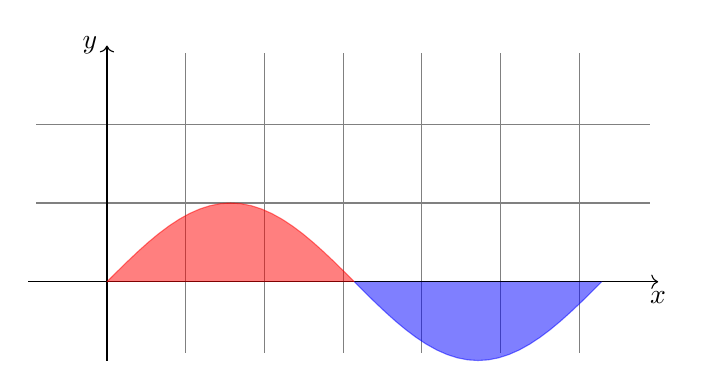
\begin{tikzpicture}
\draw[gray] (-0.9,-0.9) grid (6.9,2.9);
\draw[->] (-1,0)--(7,0) node[below]{$x$};
\draw[->] (0,-1)--(0,3) node[left]{$y$};
\filldraw[red,opacity=0.5] plot[domain=0:3.1415] (\x,{sin(180*\x/3.1415)});
\filldraw[blue,opacity=0.5] plot[domain=0:3.1415] (3.1415+\x,{-sin(180*\x/3.1415)});
\end{tikzpicture}
%$\int_0^{2\pi} \sin(x)dx=\bigg /_0^{2\pi} -\cos(x)=$

\section{Numeerista derivointia ja integrointia}
\subsection{Numeerista derivointia}

Funktion $f$ derivaatta pisteessä $x$ on määritelmän mukaan
$$
f'(x)=\lim_{h\to 0}\frac{f(x+h)-f(x)}{h}.
$$
Jos $h\approx 0$, niin
$$
f'(x)\approx \frac{f(x+h)-f(x)}{h}
$$
eli murtolauseketta (erotusosamäärä eli etenevä differenssi) voidaan käyttää derivaatan arvioimiseen.\\

\textbf{Esimerkki.} Arvioidaan funktion $f(x)=\sin(3x)$ derivaattaa pisteessä $x=1$. Valitaan $h=0.01$. Nyt $x+h=1.01$. Sijoittamalla lukuarvot ylläolevaan kaavaan saadaan
$$
f'(x)\approx\frac{\sin(3\cdot 1.01)-\sin(3\cdot 1)}{0.01}
=0.536.
$$

Alla olevissa tehtävissä laske derivaatalle likiarvo kaavalla
$$
f'(x)\approx \frac{f(x+h)-f(x)}{h},
$$
missä $x$ on tarkastelupiste ja $h=0.01$.

\begin{enumerate}
\item (Viikolta 2) Olkoon $f(x)=x^2-1$. Laske numeerisesti
\begin{enumerate}
\item $f'(x)$, ohita\ratkaisu{$2x$}
\item $f'(-2)$\ratkaisu{$-4$}
\item $f'(-1)$\ratkaisu{$-2$}
\item $f'(0)$\ratkaisu{$0$}
\item $f'(1)$\ratkaisu{$2$}
\item $f'(2)$\ratkaisu{$4$}
\end{enumerate}
\item (Viikolta 3) Olkoon $f(x)=2^x$. Laske numeerisesti
\begin{enumerate}
\item $f'(x)$, ohita\ratkaisu{$2^x\ln(2)$}
\item $f'(0)$\ratkaisu{$\ln(2)\approx 0.7$}
\item $f'(1)$\ratkaisu{$1.4$}
\item $f'(2)$\ratkaisu{$2.8$}
\item $f'(-1)$\ratkaisu{$0.35$}
\item $f'(-2)$\ratkaisu{$0.175$}
\end{enumerate}
\end{enumerate}

\newpage
\subsection{Numeerista integrointia}

Integraalia voidaan arvioida vasemman päätepisteen menetelmällä
$$
\int_a^b f(x)dx
\approx V=\sum_{k=1}^{N} f(x_{k-1})(x_k-x_{k-1})
$$
oikean päätepisteen menetelmällä
$$
\int_a^b f(x)dx
\approx O=\sum_{k=1}^{N} f(x_k)(x_k-x_{k-1})
$$
puolisuunnikasmenetelmällä
$$
\int_a^b f(x)dx
\approx P=\sum_{k=1}^{N} \frac{f(x_k)+f(x_{k-1})}{2}(x_k-x_{k-1})
$$
ja keskipistemenetelmällä
$$
\int_a^b f(x)dx
\approx K=\sum_{k=1}^{N} f\brac{\frac{x_k+x_{k-1}}{2}}(x_k-x_{k-1}).
$$
Tässä pätee $P=(V+O)/2$. Simpsonin menetelmä on $S=(P+2K)/3$. \textbf{On hyvä tietää, että erilaisia menetelmiä on olemassa.} Kuitenkin usein jokin yksinkertainen menetelmä (esim. vasemman päätepisteen menetelmä) on sovelluksissa ihan OK. Tietokoneella askelpituuden $x_k-x_{k-1}$ saa asetettua tarvittavan pieneksi.

Helpointa on laittaa jakopisteet $x_k$ tasavälisesti kaavalla
$$
x_k=a+(b-a)\frac{k}{N}.
$$

\textbf{Esimerkki.} Tiedetään, että
$$
\int_0^\pi \sin(x)dx=2.
$$
Lasketaan tämä numeerisesti kahdella tavalla

(a) WolframAlphalla komennolla

\begin{verbatim}
sum k=1 to k=100 sin(x)*w where x=a+(b-a)*k/100 and w=(b-a)/100 and a=0 and b=pi
\end{verbatim}

linkki \url{https://www.wolframalpha.com/input?i=sum+k%3D1+to+k%3D100+sin%28x%29*w+where+x%3Da%2B%28b-a%29*k%2F100+and+w%3D%28b-a%29%2F100+and+a%3D0+and+b%3Dpi}

tulos on 1.99984.

(b) Octave-koodilla (asenna Octave tai käytä OctaveOnlinea \url{https://octave-online.net/})

\begin{verbatim}
format long
a=0;
b=pi;
N=100;
dx=(b-a)/N;
s=0;
for k=1:100
x=a+(b-a)*k/N;
s=s+sin(x)*dx;
end
s
\end{verbatim}

lopputulos on $s=1.999835503887444$, joka antaa pyöristettynä $s=1.99984$.\\

Alla olevissa tehtävissä käytä jompaa kumpaa menetelmää. Integraalit ovat alkukurssilta tuttuja.

\begin{enumerate}
\setcounter{enumi}{2}
\item (Viikolta 2) Laske integraalit.
\begin{enumerate}
\item $\int_0^2 xdx$\ratkaisu{$2$}
\item $\int_0^2 x^2dx$\ratkaisu{$\frac83$}
\item $\int_0^2 x^3dx$\ratkaisu{$4$}
\item $\int_0^3 \sqrt{x}dx$\ratkaisu{$2\sqrt{3}\approx 3.464.$}
\end{enumerate}
\item (Viikolta 3) Laske integraalit.
\begin{enumerate}
\item $\int_0^2 2^xdx$\ratkaisu{$4.3281$}
\item $\int_0^2 3^xdx$\ratkaisu{$7.2819$}
\item $\int_0^2 0.5^xdx$\ratkaisu{$1.082$}
\end{enumerate}
\item (Viikolta 5) Laske integraalit.
\begin{enumerate}
\item $\int_0^\pi \sin(x)dx$\ratkaisu{$2$}
\item $\int_{-\frac{\pi}{2}}^{\frac{\pi}{2}} \cos(x)dx$\ratkaisu{$0$}
\item $\int_0^{2\pi} \sin(x)dx$\ratkaisu{$0$}
\end{enumerate}
\end{enumerate}

\newpage
\subsection{Taylorin sarja}

Derivoinnin sovelluksena voidaan etsiä polynomi, joka on lähellä annettua funktiota.

Taylorin sarja on kaava
$$
f(x)=\sum_{n=0}^\infty \frac{f^{(n)}(a)}{n!}(x-a)^n.
$$
Merkintä $f^{(n)}$ tarkoittaa funktiota $f$ derivoituna $n$ kertaa. Merkintä $n!$ tarkoittaa luvun $n$ kertomaa, joka on $1\cdot 2\cdot 3\cdot\ldots\cdot (n-1)\cdot n$. Pätee $0!=1$ ja $1!=1$.

Usein asetetaan $a=0$ (ns. Maclaurin sarja). Saadaan helpompi kaava
$$
f(x)=\sum_{n=0}^\infty \frac{f^{(n)}(0)}{n!}x^n.
$$
Sarjassa on äärettömän monta termiä, esimerkiksi
$$
e^x=1+x+\frac{x^2}{2}+\frac{x^3}{6}+\frac{x^4}{24}+\ldots.
$$
Katkaisemalla sarja jostakin kohtaa saadaan funktiota arvioiva Taylorin polynomi, esimerkiksi
$$
e^x\approx 1+x+\frac{x^2}{2},\quad\textrm{kun}\quad x\approx 0.
$$
Taylorin polynomien avulla voidaan näppärästi määritellä funktioita ohjelmistoihin ja laskea likiarvoja.

\textbf{Esimerkki.} Arvioi integraalia
$$
\int_0^{1} e^{x}dx
=\sij{0}{1} e^x=e^1-e^0 \approx 1.71828.
$$
korvaamalla eksponenttifunktio Taylorin polynomilla
$$
e^x\approx 1+x+\frac{x^2}{2}+\frac{x^3}{6}.
$$
\textbf{Ratkaisu.} Saadaan
$$
\int_0^1 1+x+\frac{x^2}{2}dx
=\bigg/_0^1 x+\frac{x^2}{2}+\frac{x^3}{2\cdot 3}+\frac{x^4}{6\cdot 4}
=1+1^2/2+1^3/6+1^4/24
=1.708333
$$
Virhe on noin $0.01$.

\textbf{Esimerkki.} Arvioi integraalia
$$
\int_0^{1} e^{x^2}dx\approx 1.46265.
$$
korvaamalla eksponenttifunktio Taylorin polynomilla
$$
e^t\approx 1+t+\frac{t^2}{2}.
$$
\textbf{Ratkaisu.} Sijoitetaan $t=x^2$ lausekkeeseen
$$
e^t\approx 1+t+\frac{t^2}{2},
$$
saadaan
$$
e^{x^2}\approx 1+x^2+\frac{x^4}{2}.
$$
Siis
$$
\int_0^1 1+x^2+\frac{x^4}{2}
=\bigg /_0^1 x+\frac{x^3}{3}+\frac{x^5}{10}
=1+1/3+1/10\approx 1.4333.
$$
Virhe on noin $0.03$.

Taylorin sarjoja löytyy esim. sivulta \url{https://fi.wikipedia.org/wiki/Taylorin_sarja}.

\begin{enumerate}
\setcounter{enumi}{5}
\item (Vapaaehtoinen.) Arvioi integraaleja käyttämällä sopivaa Taylorin sarjaa.  
\begin{enumerate}
\item $\int_0^1\sin(x^2)dx=0.310268\ldots$\ratkaisu{Esimerkiksi $$\int_0^1 x^2-\frac{x^6}{6}+\frac{x^{10}}{120}dx\approx 0.31028.$$}
\item $\int_0^1\cos(x^2)dx=0.9045\ldots$\ratkaisu{Esimerkiksi $$\int_0^1 1-\frac{x^4}{2}dx=0.9$$}
\item $\int_0^1\arctan(x^2)dx=0.2979\ldots$\ratkaisu{Esimerkiksi $$
\int_0^1 x^2-\frac{x^6}{3}dx\approx 0.2857.
$$}
\end{enumerate}
\end{enumerate}

\end{document}